\chapter{Methods}\label{chap:methods}

% \epigraph{Elections do not take place on the pages of academic books but in the
% real world.}{The International IDEA Handbook of Electoral System Design}

This work designs, builds, and analyzes various electoral systems, electoral
features, and voter authentication models. Implementations are provided as smart
contracts which are used to determine their efficacy, feasibility, and usability
as tools to aid in on-chain decision-making processes.

It is undeniable that the underlying infrastructure and properties thereof,
which are intrinsic to blockchain technologies, present risks and weaknesses
with regard to voting; however, these properties also present unique
opportunities to explore non-traditional and novel approaches to governance
models, mechanisms, and electoral systems. This research aims to lean into the
advantages of the intrinsic properties made available by blockchain
technologies, while attempting to minimize the risks presented and weaknesses
exposed which are derived alongside them.

% offers the potential to explore non-traditional governance models and
% mechanisms, e.g., delegative democracies. This research aims to explore some of
% these non-traditional governance models and in general aims to lean into what
% advantages are made available through the underlying technologies while
% attempting to minimize the weaknesses and risks they present.

% The infrastructure provided by blockchain technology offers the potential to
% explore non-traditional governance models and mechanisms, e.g., delegative
% democracies. This research aims to explore some of these non-traditional
% governance models; and lean into what advantages are made available by
% the underlying technologies while attempting to minimize the
% weaknesses and risks presented by these blockchain technologies.
%
% Internet voting and blockchain technologies offer opportunities to approach
% governance in new and novel ways; explore non-traditional governance models
% like delegative and liquid democracies.
%
% would be infeasible explore models of governance in ways that have been would be
% other non-traditional and approach governance in non-traditional ways.
%
% Consideration must be paid to the limitations of the Ethereum Virtual Machine
% and Ethereum network, namely cost of storage, cost of computation, and
% limitations in regards to computation per block.
%
% Some electoral systems can be tallied through a simple summation of votes across
% choices, others must be tallied in multiple stages multiple times across
% pairwise combinations of simulated elections. Electoral systems which require
% the latter fare better in centralized systems where the cost of computation is
% less expensive.

% FIXME: Too Opinionated
%   Change `slaves to` to `bound by`.

% , we need not be bound by
% traditional electoral systems. Indeed, it is likely that the electoral systems
% that we are used to dealing with as citizens of monolithic and centralized
% governments are not appropriate for the fragmented crypto-anarchistic leaning
% groups of blockchain enthusiasts who are likely to participate in these
% decentralized organizations and communities.


% Section: Requirements
\section{Requirements}\label{sec:requirements}
Borrowing from the requirements introduced and defined by, ``The Future of
Voting: End-to-End Verifiable Internet Voting''\cite{e2e-viv} --- which were
outlined in Chapter~\ref{chap:literature}, \emph{\nameref{chap:literature}}, and
grouped into two major categories: technical and non-functional --- a set of
requirements are identified and targeted for satisfaction. These requirements
provide a framework to analyze the results produced by this research.
Table~\ref{tab:research-requirements} summarizes the requirements targeted for
fulfillment.

% % \NewDocumentCommand{\vgood}{ O{\cmark} }{\cellcolor{green!40}#1}
% % \begin{minipage}[t]{1\linewidth}
%   \begin{minipage}[t]{0.50\textwidth}
%     \begin{enumerate}[label=, leftmargin=0mm, topsep=2mm, align=left]
%       % \small
%       \normalsize
%       \item \textbf{Technical Requirements}
%       \item[\faCheck]        authentication requirements
%       \item[\faCheck]        system operational requirements
%       \item[\faPlus]         reliability requirements
%       \item[\faPlus]         security requirements
%       \item[\faPlus]         auditing requirements
%       \item[\faPlus]         functional requirements
%       \item[\faMinus]        interoperability requirements
%       \item[\faMinus]        certification requirements
%       \item[\faRemove]       accessibility requirements
%       \item[\faRemove]       usability requirements
%     \end{enumerate}
%   \end{minipage}
%   \begin{minipage}[t]{0.50\textwidth}
%     \begin{enumerate}[label=, leftmargin=0mm, topsep=2mm, align=left]
%       % \small
%       \normalsize
%       \item \textbf{Non-Functional Requirements}
%       \item[\faPlus]         maintenance/evolvability requirements
%       \item[\faPlus]         assurance requirements
%       \item[\faRemove]       operational requirements
%       \item[\faRemove]       procedural requirements
%       \item[\faRemove]       legal requirements
%     \end{enumerate}
%   \end{minipage}\\
%   % \begin{multicols}{2}
%   % \begin{itemize}[label=,leftmargin=7mm,topsep=-40mm]
%   \begin{itemize}[label=, leftmargin=0mm, topsep=3mm]
%     % Reduce item separation.
%     % \setlength\itemsep{-5mm}
%     \scriptsize
%     \footnotesize
%     \item[\faCheck]        Requirements which are targeted to be \emph{fully} satisfied.
%     \item[\faPlus]         Requirements which are targeted to be \emph{mostly} satisfied.
%     \item[\faMinus]        Requirements which are targeted to be \emph{partially} satisfied.
%     \item[\faRemove]       Requirements which are expected to remain \emph{unsatisfied}.
%   \end{itemize}
%   % \end{multicols}
% % \end{minipage}

\begin{spacing}{1.1}
  \begin{longtabu} to \textwidth{X[0.1,l] X[2.3,j] X[0.8,c] X[0.8,c] X[0.8,c] X[1.1,c]}
    % \multicolumn{2}{c}{Requirements} \\
    \caption{Requirements targeted for fulfillment.} \\
    \toprule
    \multicolumn{2}{l}{{Requirements}}                                       & \multicolumn{3}{c}{Targeted}                  & {Untargeted} \\
                                                                               \cmidrule{3-5}
    \multicolumn{2}{l}{}                                                     & {Fully}       & {Mostly}       & {Partially}  &               \\
    \midrule
    \endhead
    \multicolumn{2}{l}{\emph{Technical}} \\
    % \addlinespace[-0.4ex]
    % \cmidrule(lr){1-2} \cmidrule(lr){3-5} \cmidrule(lr){6-6}
    % \addlinespace[-0.4ex]
    % \cline{1-2}
    % \midrule
    % \multirow{10}{*}{\rot[90]{Technical}}     & Authentication               & \textbullet{} &                &               &               \\
                                              & Authentication               & \textbullet{} &                &               &               \\
                                              & System Operational           & \textbullet{} &                &               &               \\
                                              & Reliability                  &               & \textbullet{}  &               &               \\
                                              & Security                     &               & \textbullet{}  &               &               \\
                                              & Auditing                     &               & \textbullet{}  &               &               \\
                                              & Functional                   &               & \textbullet{}  &               &               \\
                                              & Interoperability             &               &                & \textbullet{} &               \\
                                              & Certification                &               &                & \textbullet{} &               \\
                                              & Accessibility                &               &                &               & \textbullet{} \\
                                              & Usability                    &               &                &               & \textbullet{} \\
    % \midrule
    % \cmidrule(lr){1-2} \cmidrule(lr){3-5} \cmidrule(lr){6-6}
    \addlinespace[0.4ex]
    \cmidrule(lr){1-2} \cmidrule(lr){3-5} \cmidrule(lr){6-6}
    \multicolumn{2}{l}{\emph{Non-Functional}} \\
    % \cline{1-2}
    % \cmidrule{1-2}
    % \midrule
    % \multirow{5}{*}{\rot[90]{Non-Functional}} & Maintenance/Evolvability     &               & \textbullet{}  &               &               \\
                                              & Maintenance/Evolvability     &               &                & \textbullet{} &               \\
                                              & Assurance                    &               &                & \textbullet{} &               \\
                                              & Operational                  &               &                &               & \textbullet{} \\
                                              & Procedural                   &               &                &               & \textbullet{} \\
                                              & Legal                        &               &                &               & \textbullet{} \\
    \bottomrule\label{tab:research-requirements}
  \end{longtabu}
\end{spacing}

The requirements identified in ``The Future of Voting: End-to-End Verifiable
Internet Voting'' have rightfully demanding and difficult to meet criteria for
fulfillment; however, the expectations laid out for a system of the kind
imagined in the study are far beyond the scope of this research. Therefore, a
subset of the technical and non-functional requirements are identified which
are considered achievable, relevant, and within the scope of this research. The
requirements are individually assessed and categorized based on whether their
criteria for satisfaction are considered feasible to fully, mostly, or partially
satisfy. The remaining requirements are considered either outside of the scope
of this research or not feasible to otherwise fulfill and are therefore not
targeted. Several requirements are identified which are considered partially or
mostly satisfied by virtue of intrinsic properties made available through the
underlying blockchain technology.

% \begin{center}
% \begin{spacing}{1.5}
%   \begin{longtabu} to \textwidth{ X[1] X[1] }
%     % \multicolumn{2}{c}{Requirements} \\
%     \toprule
%     {Technical Requirements}        & {Non-Functional Requirements}        \\
%     \midrule
%     \endhead
%     \faCheck{}  authentication      & \faPlus{}   maintenance/evolvability \\
%     \faCheck{}  system operational  & \faPlus{}   assurance                \\
%     \faPlus{}   reliability         & \faRemove{} operational              \\
%     \faPlus{}   security            & \faRemove{} procedural               \\
%     \faPlus{}   auditing            & \faRemove{} legal                    \\
%     \faPlus{}   functional          &                                      \\
%     \faMinus{}  interoperability    &                                      \\
%     \faMinus{}  certification       &                                      \\
%     \faRemove{} accessibility       &                                      \\
%     \faRemove{} usability           &                                      \\
%     \bottomrule
%   \end{longtabu}
% % \begin{multicols}{2}
%   \begin{itemize}[label=,leftmargin=0mm,topsep=0mm]
%     % Reduce item separation.
%     % \setlength\itemsep{-5mm}
%     \scriptsize
%     \footnotesize
%     \item[\faCheck]        Requirements which are targeted to be \emph{fully} satisfied.
%     \item[\faPlus]         Requirements which are targeted to be \emph{mostly} satisfied.
%     \item[\faMinus]        Requirements which are targeted to be \emph{partially} satisfied.
%     \item[\faRemove]       Requirements which are expected to remain \emph{unsatisfied}.
%   \end{itemize}
% % \end{multicols}
% \end{spacing}
% \end{center}

\subsection{Technical Requirements}
The technical requirements are requirements which the study asserts should be
fulfilled through the design and architecture of the system. This research
attempts to fully satisfy the authentication and system operational
requirements; considers the accessibility and usability requirements beyond the
scope of this research, and therefore makes no effort to satisfy them; and
targets partial satisfaction of the remaining requirements. Requirements which
are targeted to be partially satisfied are reviewed in further detail.

\paragraph{Reliability and Security Requirements}
Reliability and security requirements are considered \emph{mostly} satisfiable
due to the inherent properties made available by Ethereum and its decentralized
structure; however, there are some notable potential attacks on the network
which are worth considering; these are discussed in further detail in
Chapter~\ref{chap:results}, \emph{\nameref{chap:results}}.

\paragraph{Auditability Requirements}
Ethereum inherently offers a tremendously detailed log through its blockchain
structure which provides a wide range of opportunities for detailed auditing and
validation. Furthermore, auditing and validation functionality are inherent
features of the blockchain. However, the auditability which Ethereum provides is
not considered a privacy preserving feature and therefore falls short of the
criteria presented.

\paragraph{Functional Requirements}
A subset of the functional requirements are deemed relevant to this research:

\begin{itemize}[topsep=0pt]
  \item[\faCheck] Multi-vote functionality is targeted to be investigated and
    fully satisfied in all electoral system implementations.
    % However, the receipt freedom which it is generally meant to reflect is not
    % satisfied along with it.

  \item[\faPlus] Ensuring that ``a voter's ballot, and the act of them casting a
    ballot, is recorded and retained as expected;'' is considered \emph{mostly}
    fulfilled through intrinsic properties of the Ethereum blockchain. Where
    this property falls short is when a voter casts a ballot, broadcasts a
    transaction to the network, which miners fail to include in any blocks. This
    is discussed further in Chapter~\ref{chap:results},
    \emph{\nameref{chap:results}}.

  \item[\faMinus] Maintaining voter anonymity is considered \emph{partially}
    fulfilled through intrinsic properties of the Ethereum blockchain. While it
    is \emph{technically} possible to broadcast privacy-maintaining
    transactions, those which preserve anonymity on the Ethereum network, it is
    likely beyond the capabilities of most voting actors and would be difficult
    to guarantee in any meaningful way. Pseudo-anonymity is a better profile of
    the kind of anonymity which Ethereum offers, This is discussed further in
    Chapter~\ref{chap:results}, \emph{\nameref{chap:results}}.
\end{itemize}

\subsection{Non-Functional Requirements}
The non-functional requirements are those which the study asserts must be
fulfilled by entities external to the system itself. These requirements are
regarded as being mostly beyond the scope and context of this research, however,
the existence of this document does itself at least \emph{partially} satisfy
some of the categories of requirements, e.g., assurance, maintenance, and
evolvability. Detailed documentation regarding design, architecture and
implementation is provided in Appendix~\ref{appendix:documentation},
\emph{\nameref{appendix:documentation}}.


% Section: Assumptions and Objectives
\section{Assumptions and Objectives}\label{sec:objectives}
Given the nascent nature of blockchain technologies, it is difficult to imagine
the demands and needs of the organizations and communities which will come to
exist in these cyberspace environments; and therefore difficult to predict which
governance models and electoral systems would best support them. However, it
seems likely that the needs of these organizations will vary as dramatically by
organization as the organizations which have come to exist in meatspace
environments. It therefore follows that a wide range of kinds of electoral
systems should exist which would serve to support the various governance models
and decision-making processes that are likely to form over time. Given these
assumptions, and in compliance with the aforementioned requirements, \emph{the
objectives of this research are defined as follows}:

\begin{enumerate}[topsep=0mm, leftmargin=*]
  \item This research aims to explore various electoral systems and features,
    using the content reviewed in Section~\ref{sec:elections} as a basis for
    exploration.

    \begin{enumerate}
      \item Provide a range of kinds of electoral contracts using
        Table~\ref{tab:electoral-systems} and
        Table~\ref{tab:criteria-compliance} as the primary resource for
        electoral system and feature selection.

        \begin{enumerate}
          \item Support single-winner elections and provide plurality and
            majority electoral system in fulfillment of that objective.

            \begin{enumerate}
              \item Implement first-past-the-post to fulfill the targeted
                single-winner plurality electoral system, due mostly to the fact
                that it is extremely simple, well-understood, and
                widely-adopted.

              \item Implement range vote to fulfill the targeted single-winner
                majority electoral system, due to its effectiveness and
                simplicity.
            \end{enumerate}

          \item Support multi-winner elections and provide an electoral system
            which offers proportional representation; Single transferable vote
            is selected as the electoral system implementation to fulfill both
            objectives due to its wide-adoption, prevalence, and effectiveness
            as a PR system.
        \end{enumerate}

      \item Explore the design, implementation, and efficacy of various ballot
        types across the various electoral systems selected.
    \end{enumerate}

  \item This research aims to explore voter authentication, registration, and
    access control patterns for managing voter registration.

  \item This research aims to explore delegative or liquid governance models.
\end{enumerate}


% Section: Tooling
\section{Tooling}
As mentioned in Section~\ref{eth:evm}, Ethereum offers a code execution
environment via the Ethereum Virtual Machine. The EVM is responsible for
executing a set of low-level instructions which can be used to update the state
of the network.\cite{ethereum-yellow} A number of higher-level languages exist
that are capable of being compiled into the low-level bytecode representation
required by the EVM for execution; this research uses the Solidity language. In
order for the EVM to execute bytecode, it must first exist on the Ethereum
blockchain. Deployment of bytecode to the Ethereum blockchain is performed by
constructing, and submitting to the Ethereum network, an account creation
transaction which includes the EVM bytecode. The account creation transaction
instructs the EVM to create a new account and to store the included bytecode
within it. Upon receiving the account creation transaction the EVM will execute
a special {\tiny{CREATE}} instruction (see Table~\ref{tab:gas-costs}) which
will eventually result in the creation of an ``internal account.'' This
internal account will contain the EVM bytecode, submitted with the create
account transaction, and is commonly referred to as a ``smart contract.'' Once
a smart contract exists on Ethereum blockchain, the bytecode stored within it
can be executed by constructing and submitting another transaction to the
network; this time instructing the EVM to execute the bytecode stored within
the smart contract. Beyond the bytecode stored in them when created, smart
contracts also contain and maintain their own internal state on the network,
which they can use as storage.

\subsection{Frameworks}
Given the complex process involved in compiling and deploying smart contracts to
the Ethereum network, a framework is typically leveraged to simplify development
and manage the smart contract deployment life-cycle. This research leveraged two
different software frameworks to aid in the development of smart contracts:
Embark and Truffle. Both of these frameworks aid in the compilation of Solidity
code, deployment of EVM bytecode, provisioning of test networks, and testing of
contract functionality.

\subsubsection{Embark}
Initially, smart contract implementations were built using the Embark framework.
The Embark framework is designed to aid in the construction and deployment of
Decentralized Applications (DApps); it supports functionality to provision test
networks, build and deploy contract code, and execute tests against deployed
smart contracts. The Embark framework is capable of managing, and deploying
contracts to, various other Ethereum blockchains; e.g., the testnet, private
net, and livenet. The Embark framework supports several useful development
features. For example, Embark can be configured to detect changes to contract
code during development, then trigger a recompilation and redeployment of
modified contract code to the appropriate Ethereum networks.

To build Solidity code into EVM bytecode, the Embark framework leverages
\solt{solcjs}, which offers JavaScript bindings for the Solidity compiler. For
expedited development and testing, Embark exposes the Ethereum JavaScript
\solt{testrpc}. The \solt{testrpc} simulates a fully functioning Ethereum
client, features an API for programmatic interaction (a useful feature during
test execution), and is capable of transaction execution speeds that complete
near-instantaneously (speeds which could not be matched by a live Ethereum
network). Embark simplifies interaction with Ethereum contracts by generating
contract-equivalent (promise-based) JavaScript functions that can be called to
execute contract code. JavaScript support is provided by wrapping the
\solt{web3js} library which implements the generic Ethereum JSON RPC spec.

The Embark framework also boasts support for other tools useful for building
decentralized applications; decentralized storage support via IPFS,
decentralized messaging functionality via Whisper and Orbit, and a curses-like
dashboard which exposes logs, environment configuration, contract state, service
availability, the status of application components and dependencies, and
features an interactive console for executing commands and querying application
state. A screenshot of the Embark dashboard is shown in
Figure~\ref{fig:embark-dashboard}.

\begin{figure}[H]
  \centering
  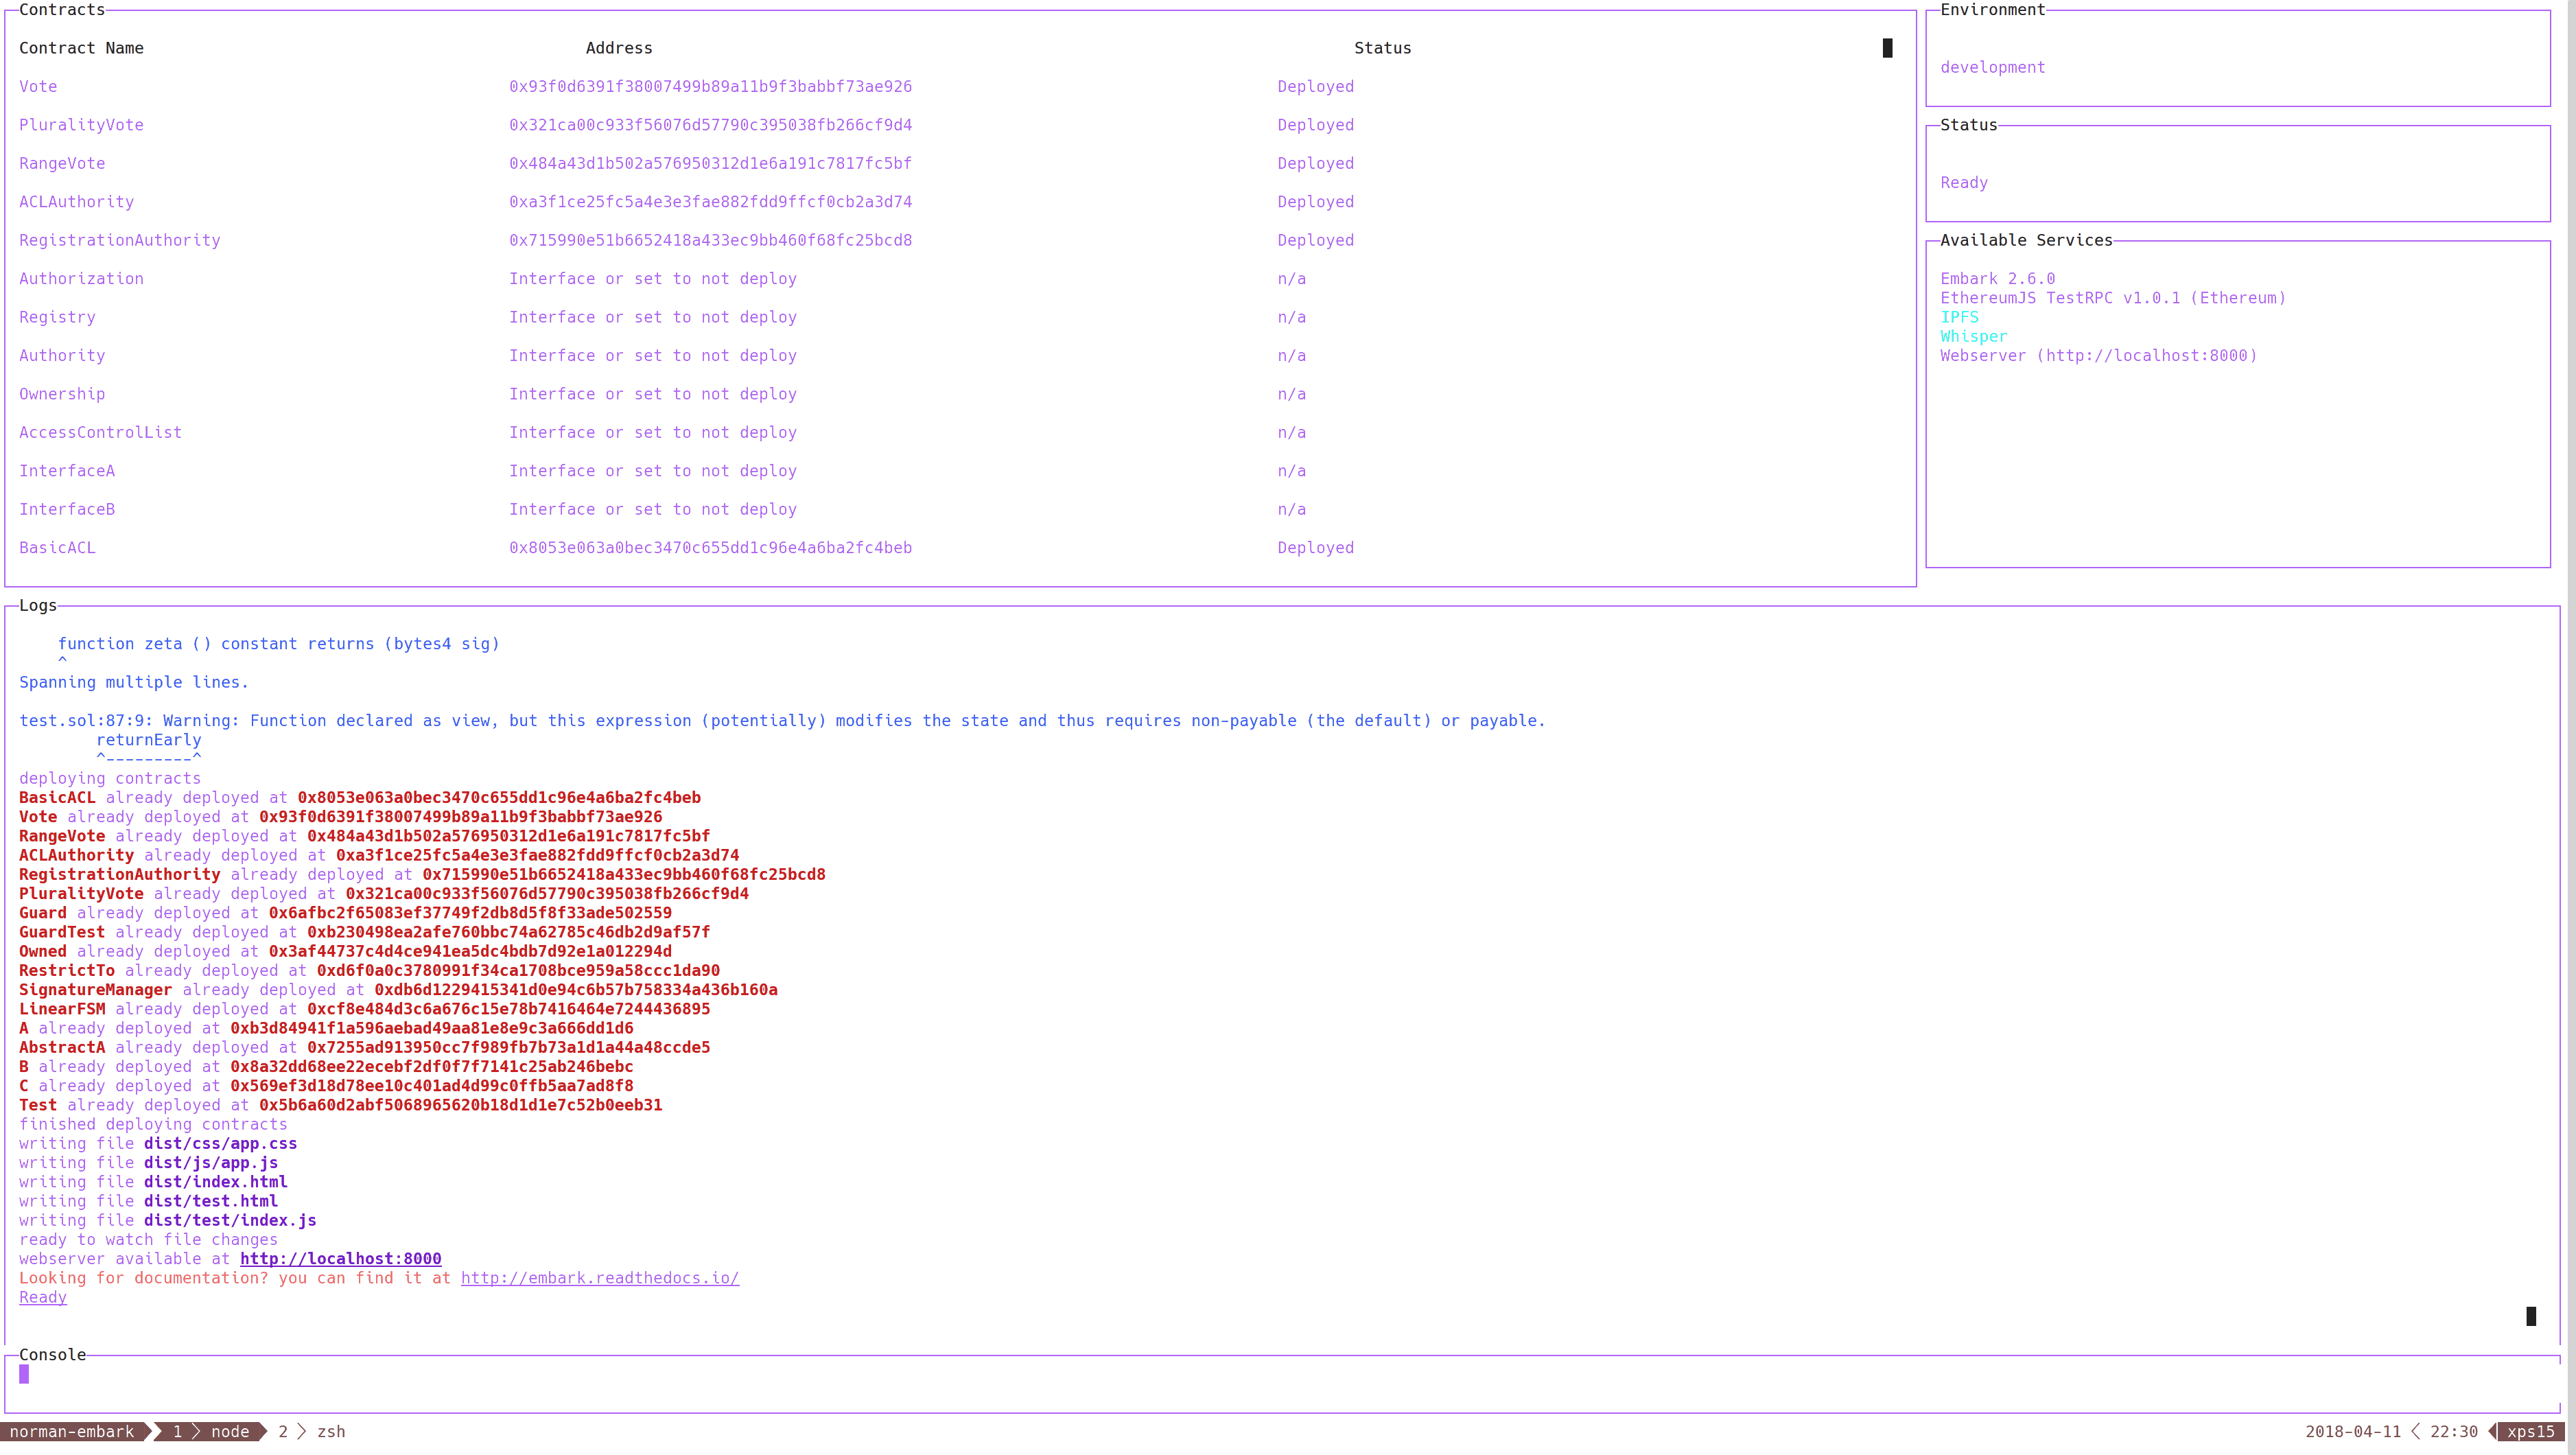
\includegraphics[width=\textwidth]{embark-ui-transparent-bg}
  \caption{The Embark dashboard and application state.}\label{fig:embark-dashboard}
\end{figure}


\subsubsection{Truffle}
Later smart contract development was completed using the Truffle framework. When
compared to the contract development features of the Embark Framework, the
Truffle framework can be viewed as an almost feature-identical framework ---
i.e., smart contract lifecycle management, testing functionality, JavaScript
bindings, and network management --- however, unlike the Embark framework, the
Truffle framework offers essentially no features related to DApp development.
The Truffle framework's more targeted focus with regards to smart contract
development and management produced a cleaner development experience during the
pursuit of this research, which is concerned strictly with smart contract design
and implementation and not DApp development. Furthermore, the Truffle framework
supports executing workflows and tests in TypeScript, and can be used in
conjunction with \solt{TypeChain} to generate TypeScript types for use with the
smart contract bindings generated by Truffle. A screenshot displaying the
execution of a contract test via the Truffle framework can be seen in
Figure~\ref{fig:truffle-test}.

\begin{figure}[H]
  \centering
  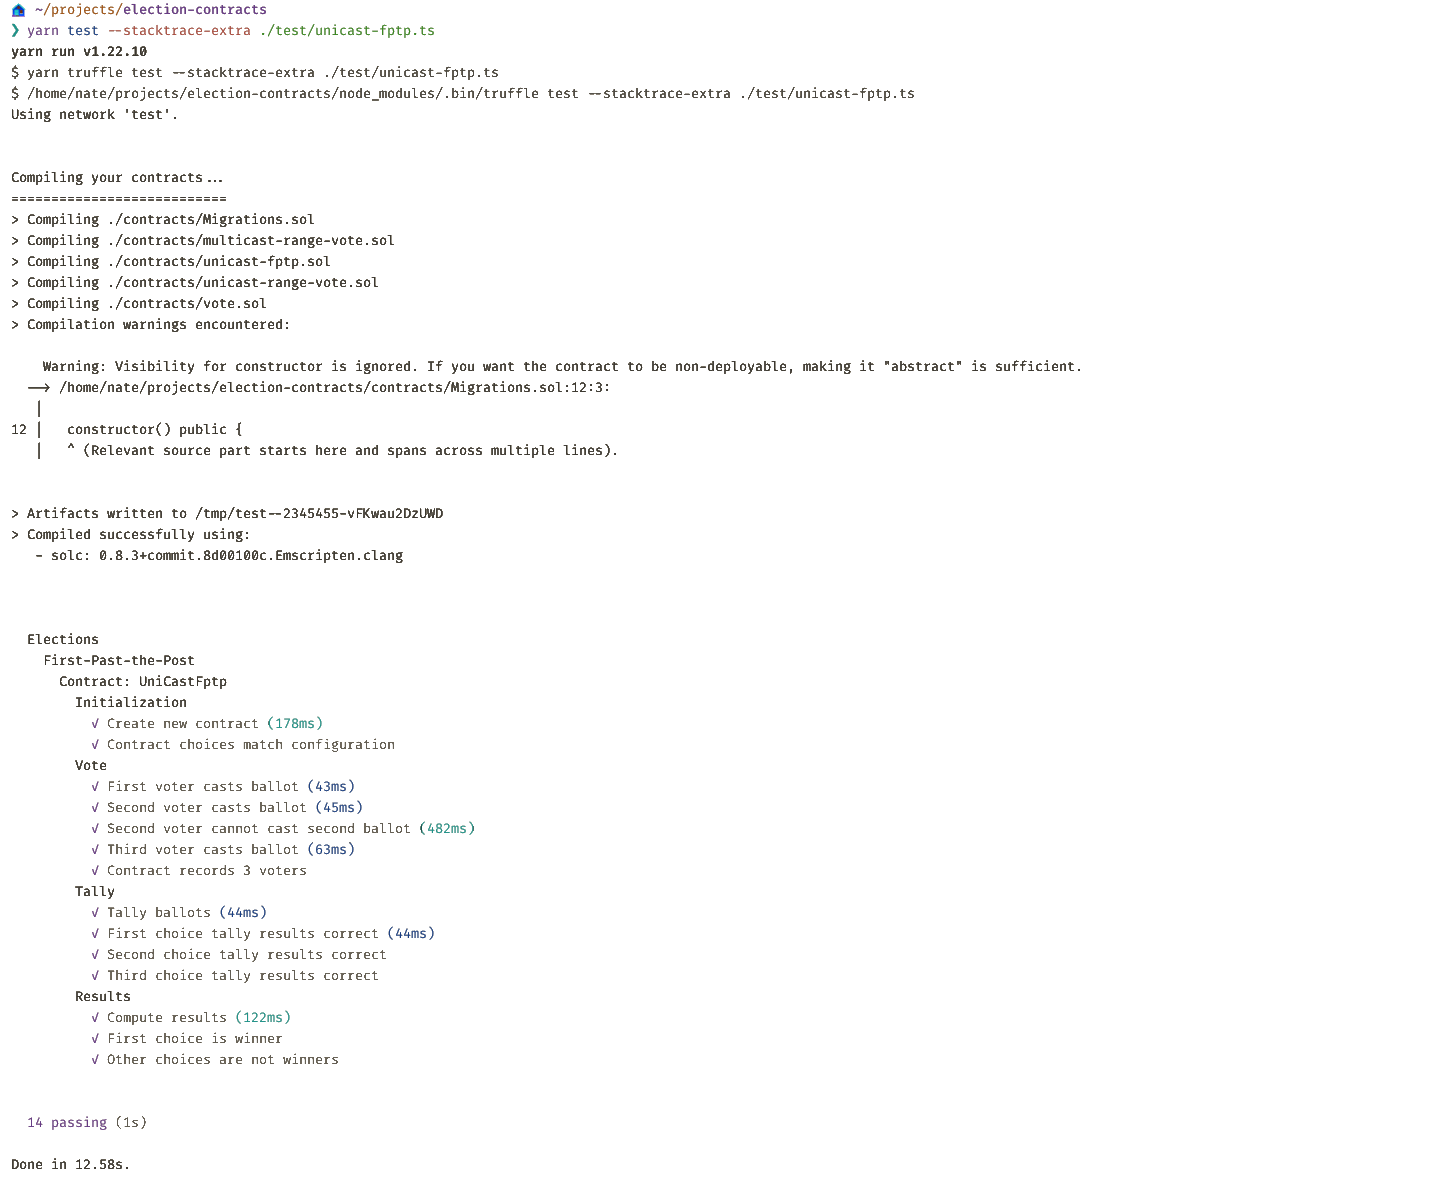
\includegraphics[width=\textwidth]{truffle-test-transparent-bg}
  \caption{Testing an election contract using the Truffle framework.}\label{fig:truffle-test}
\end{figure}

% seemed to result in to  i.e., lifecycle management, contract testing and
% debugging,


% Section: Design
\section{Architecture and Design}\label{sec:architecture-and-design}
The design of the system is approached in three phases: authorization, election,
and delegation. Each phase considers different components of the overall system
architecture and each component is responsible for managing a different set of
responsibilities within the architecture.

% system. The authorization components, delegation components, and election
% components.

% , henceforth collectively referred to as Norman.

% The Embark framework --- a framework designed to build Decentralized
% Applications (DApps) --- is used to provision test networks, build, deploy,
% and test the components. The Embark framework can manage and deploy to
% different chains, e.g., testnet, private net, and livenet. Embark
% automatically detects changes to contracts, builds, and then deploys the
% contracts onto the appropriate Ethereum networks. To build Solidity code into
% EVM code the Embark framework uses solcjs which offers JavaScript bindings for
% the Solidity compiler. For expedited development and testing Embark exposes
% the Ethereum JavaScript testrpc which simulates a fully functioning Ethereum
% client. Interaction with Ethereum contracts is simplified by automatically
% generating promise-based JavaScript functions which expose contract functions.
% JavaScript support is provided by wrapping the web3js library which implements
% the generic Ethereum JSON RPC spec. Embark also supports decentralized storage
% via IPFS, decentralized messaging through Whisper and Orbit, and a curses-like
% dashboard which exposes logs, environment, contract states, available
% services, a console, and the status of the framework generally.

\begin{center}
  \figurepdf{venn-diagram}
  % \includestandalone{\fig{venn-diagram}}
\end{center}

\subsection{Authorization Components}
The authorization components are designed to provide access control: to build
and maintain a set of eligible voters, administrators, and whatever other roles
might be necessary to implement the electoral systems. Ultimately, the
authorization components are responsible for restricting access to sensitive
contract function calls that mutate the state of the contract, e.g., casting
ballots and configuration elections. The design must be flexible enough to
facilitate the varying and evolving needs of different organizations and
communities but consistent enough to support them all through a common
interface. Concepts are borrowed from traditional operating system access
control schemes/models and authorization mechanisms which provide guidance for
system design. The underlying authentication features are handled via the
asymmetric cryptography provided by the underlying blockchain infrastructure.

\subsubsection{Access Control}
Access control schemes exist to authorize access to data and resources; they are
responsible for managing and defining the relationships between permissions,
operations, objects, and subjects. Several access control model schemes were
considered in this phase; among them were: access control lists, discretionary
access control, mandatory access control, and role-based access control.

\paragraph{Discretionary Access Control}
Discretionary Access Control (DAC) is a form of access control where the owner
of some resource/object can dictate the operations and permissions that other
subjects can take on the resource/object. Additionally, the owner of the
resource/object can pass ownership to some other subject. You can see a form of
this in POSIX file systems where ownership over files is granted and transferred
through commands like \codet{chown} and \codet{chmod}.

\paragraph{Access Control Lists}
An Access Control List (ACL) is a collection of \emph{subject}, \emph{resource},
and \emph{permission} relationships which can be understood as a matrix, where
each cell, indexed by \emph{subject} and \emph{resource}, reflects the
\emph{permissions} available for the \emph{subject} to access \emph{resource}.

% \todo{Intersection? Corresponding?}

\paragraph{Role-Based Access Control}
Role-Based Access Control (RBAC) is a form of access control where collections
of permissions are assigned to roles; roles are then assigned to users. In RBAC
roles are hierarchical, thus roles can be inherited from parent roles.

% Word semantic?
\subsubsection{Design}
The fundamental resources exposed by smart contracts are function calls, thus
the security implementation and access control model must revolve around that.
We define an interface, \sol{Authority}, which defines the \sol{canCall}
function. Any contract wishing to implement access control on functions can
leverage a contract that implements the \sol{Authority} interface to authorize
access to those functions.

\begin{figure}[H]
  \centering
  \figurepdf[width=\textwidth]{authorization}
  % 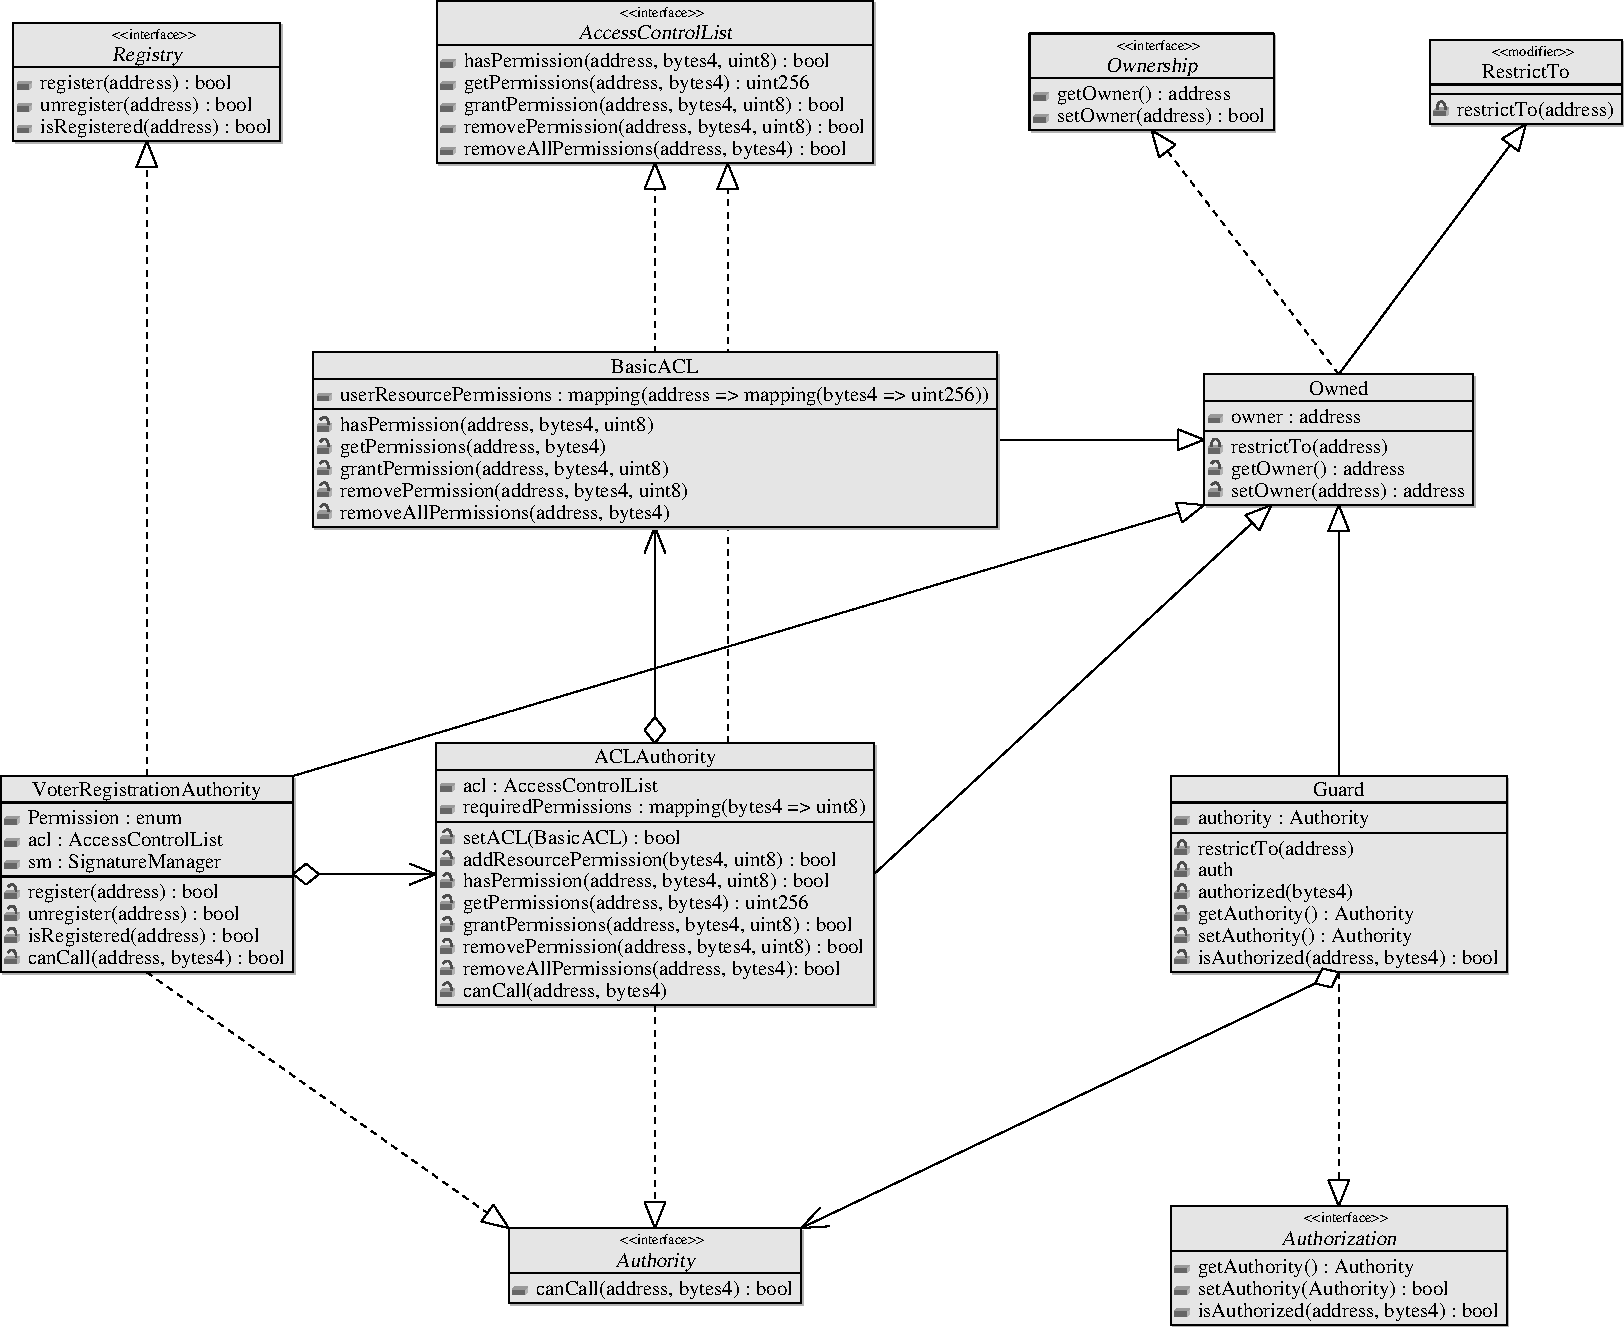
\includegraphics[width=\textwidth]{figures/authorization/figure}
  % \includestandalone[width=\textwidth]{\fig{authorization}}
  \caption{Authorization dependency graph modeling.}\label{fig:authorization}
\end{figure}

We define the \sol{Authorization} interface which offers mechanisms for
interacting with an \sol{Authority}. This interface defines \sol{getAuthority},
\sol{setAuthority}, and most importantly, \sol{isAuthorized}. A contract that
realizes the \sol{Authorization} interface is expected to aggregate an
\sol{Authority} but does not necessarily need one externally; for example, a
contract that provides \sol{Authorization} may also be its own \sol{Authority}.
Likewise, an \sol{Authority} can provide its own \sol{Authorization}. The
\sol{Authority} and \sol{Authorization} interfaces together form our access
control primitives.

The \sol{Guard} contract realizes the \sol{Authorization} interface and provides
the modifier functions \sol{auth} and \sol{authorized}. These can be applied to
other functions to easily restrict function-call access to accounts that the
\sol{Authority} has approved, e.g.,

\begin{solidity}[Guard Usage Example]
function sensitive () public auth returns (bool _success) {
  // The `auth` modifier prevents this function from being
  // called until the Authority has confirmed that the
  // the message sender has the proper privileges.
  return true;
}
\end{solidity}

This implementation conforms to a number of design principles: separation of
concerns, dependency inversion principle, open/closed principle, interface
segregation, substitution principle, and single responsibility principle.
Ultimately it provides the flexibility and resiliency necessary to build out a
wide variety of electoral systems.

\paragraph{Ownership}
Access control often starts before our \sol{Authority} and \sol{Authorization}
realizations. Most contracts offer a primitive form of access control through
\sol{Ownership}. All contracts and most contract functions are open and public
by design; thus, it is important to lock down sensitive contract functions from
deployment. A common pattern is to store the \solt{address} of the creator of a
contract as an owner in the contract state and to use that address to restrict
access to sensitive public-facing functions. More complicated ownership
mechanisms can be built using this pattern by leveraging contracts which
delegate ownership to another contract which can then define more complex access
control and management mechanisms. To facilitate in this and many other useful
patterns we introduce a simple \sol{Ownership} interface. The \sol{Ownership}
interface defines functions \sol{getOwner} and \sol{setOwner} which get and set
the account address of a contract's owners respectively.

To facilitate in restricting access of functions to a single account we also
define a contract \sol{RestrictTo} that provides a modifier function
\sol{restrictTo}. The \sol{restrictTo} modifier can be applied to any other
function and takes an account address argument; if the address of the account
calling a \sol{restrictTo} modified function does not match the argument
provided to \sol{restrictTo} (often the owner), then the function will
immediately exit and revert any changes to the contract. Finally, we realize and
extend these two contracts to form the concrete \sol{Owned} contract. This
pattern is so ubiquitous that most, if not all, concrete contracts in our
governance ecosystem will extend this contract.

\paragraph{Authority}
We need to provide access control beyond interfaces, standards, and single
account address restrictions. Our access control implementation leans towards
access control lists as a primitive that can be extended to provide other access
control mechanisms such as role-based access control. Alternatively, a contract
can realize the \sol{Authority} interface itself if ACLs are not a useful
abstraction.

\subparagraph{Access Control List}
We first define an ACL interface, \sol{AccessControlList}, which defines basic
ACL functionality: \sol{hasPermission}, \sol{getPermissions},
\sol{grantPermission}, \sol{removePermission}, and \sol{removeAllPermissions}.
The design supports assigning up to 256 unique permissions per contract
signature.

\subparagraph{Basic ACL}
Next we realize a concrete implementation of the \sol{AccessControlList}
interface named \sol{BasicACL}. \sol{BasicACL} is primarily a
database contract which creates a mapping from account address to a mapping of
functions (the first 4 bytes of their signature) to an unsigned 256-bit integer
that represents the permissions. This implementation is similar to what can be
found in POSIX compliant operating systems. In Java one might represent this
access control model as \codet{HashMap<Account, HashMap<Function,Permission>>}.

Naturally \sol{BasicACL} provides implementations for the functions defined by
\sol{AccessControlList}: \sol{hasPermission}, \sol{getPermissions},
\sol{grantPermission}, \sol{removePermission}, and \sol{removeAllPermissions}.
These work using bitwise NOT, OR, and AND operations to modify the 256-bit
unsigned integer representing permissions for a particular (account, function)
pair.

\subparagraph{ACL Authority}
We can easily build an \sol{ACLAuthority} out of our \sol{BasicACL} using the
adapter pattern and aggregation. We simply aggregate an instance of a
\sol{BasicACL} and realize the \sol{Authority} and \sol{AccessControlList}
interfaces. Finally, we lean on the \sol{hasPermission} function to implement
our \sol{canCall} function which presumably forwards our request to a
\sol{BasicACL} instance and returns the result. This structure also allows us to
implement a composite pattern and aggregate many trusted authorities into one.

\subparagraph{Voter Registration Authority}
Our final step is to use a facade to hide the more complex implementation
details from outside contracts. We introduce a \sol{VoterRegistrationAuthority}
which realizes the \sol{Registry} and \sol{Authority} interfaces.
The \sol{Registry} interface provides some nice abstractions:
\sol{register}, \sol{unregister}, and \sol{isRegistered}. We
presume the contract aggregates some number of \sol{AccessControlList}s as
a foundation for its \sol{Registry} function implementations, but does not
need to necessarily. Finally, the \sol{canCall} function leans on the
\sol{Registry} functions, specifically \sol{isRegistered} to grant
access to functions.

The end result is a clean, public, and composable voter registration authority.


\subsection{Election Components}
The election components are responsible for constructing and operating election
processes. These responsibilities include maintaining the integrity and security
of the election, handling votes, tallying ballots, and determining election
winners.

The phases typically involved in conducting an Internet-based election,
described in Section~\ref{sec:internet-voting}, are: Setup, Distribution,
Voting, Casting, Tallying, and Auditing. Responsibilities pertaining to voter
registration, which are typically handled in the Setup phase, are expected to be
managed by Authorization components. The Distribution phase, which mostly
pertains to processes such as mailing election materials to voters, is
considered outside the scope of this research and therefore ignored. The
Auditing phase, where election integrity and results are scrutinized, is assumed
to be handled and provided by the underlying features made available by
Ethereum.

% Ideally the ballots would be recorded separately from the tallying method. If
% they were we could apply different tallying methods to the same set of ballots
% and produce different results. Unfortunately it's extremely costly to store
% ballots as part of the contract state.

% We opt for first-past-the-post and range vote for single-winner elections, the
% former for its simplicity and ubiquity, the latter for its effectiveness. This
% provides an implementation of a plurality voting system and majority voting
% system.

\subsubsection{Design}
Each electoral system implementation is unique, due mostly to the unique
requirements necessitated by their underlying tallying algorithms and ballot
structures.

There are important electoral criteria worth considering when analyzing the
implementation feasibility of these electoral systems, namely, the ballot
counting criteria: summability, polynomial time, and resolvable. These electoral
criteria are significant because they impact the gas costs associated with
operating the electoral system. Table~\ref{tab:criteria-compliance} is a useful
resource when considering these electoral criteria. Both the first-past-the-post
and range vote electoral systems are a 1\textsuperscript{st}-order summable;
i.e., ballots can be tallied using a linear amount of space with respect to the
number of choices available without losing information required to complete the
tallying processes. Both also have polytime ballot counting implementations that
are linear in the number of candidates and voters. STV is not listed in the
table; however, its single-winner equivalent (IRV) is; which implies that STV
has, at best, a tallying complexity of $O(n^2)$ and a summability complexity
of $O(n!)$ with respect to the number candidates.

Gas costs must be considered when implementing, deploying, and running contract
functions on the Ethereum Virtual Machine (EVM). If gas costs are too high then
it may become infeasible for an external account to afford to execute a contract
function, e.g., the network fees become too high to vote. Another concern to
consider is that the cost to execute a contract function may become too high to
ever complete in a single block, therefore never actually complete. The most
expensive operations, by no small margin, are operations involving storage.
Therefore it is important to minimize storage usage.

% Fortunately these EVM limitations map well
% to many voting method criteria. We can lean on these criteria and the field of
% computational social choice theory broadly to restrict the set of voting systems
% to just the ones that can be feasibly implemented on the Ethereum blockchain.

\paragraph{Finite State Machine}
Several of the voting system designs use a phased approach with timed
transitions between election states: Configuration, Frozen, Vote, and Tally.
These phases can be modeled as a finite state machine where calls to various
functions trigger transitions to different stages. A modifier function can be
used to restrict access of functions to only be callable during their
appropriate state. Most of the transitions from state to state can be designed
as timed transitions which occur lazily, i.e., the check to confirm that it is
time to transition from one state to another occurs when a function is called.
The rationale for this approach is due to the fact that Ethereum offers no
mechanism to trigger code execution \emph{from within the blockchain itself};
therefore all function calls, even if called from another function or even a
function in a different contract, must ultimately have originated from a
transaction created by an externally owned account. The product of this timed
transition implementation implies that the state restriction modifier needs to
occur after the lazily evaluated timed transition modifier; i.e., first update
the current state if it should be, then validate if the function should
executed. On the other hand, if transitions are manually updated during a
function's execution then the opposite behavior should occur; i.e., first
validate if the function should be run, then update the state as required.

\subparagraph{Configuration}
The Configuration phase, as implied by the name, exists to provide election
administrators an opportunity to configure the election contract: choices,
election start/end time, etc. After the configuration is complete the
administrators can freeze the contract, preventing it from being modified
further.

\subparagraph{Frozen}
Transitioning to the Frozen phase could simply set a boolean \sol{frozen} to
true and update the phase to Frozen. The boolean \sol{frozen} should be checked
at the start of every administrative function's execution and should cause the
immediate cease of code execution if the value is true. This serves to prevent
potentially malicious election administrators from modifying an election
contract after the voting process has started; it also serves to notify external
contracts and users that the election is configured and is ready or waiting to
move into the Vote phase.

\subparagraph{Vote}
The Vote phase is the phase during which various kinds of voting can occur for a
particular election contest. A \sol{vote} function should be defined. For
flexibility, a \sol{vote (uint8[], uint8[])} function signature is considered
which is capable of being leveraged by most kinds of electoral systems and
ballot structures. For example, as a sparse vector, where both arrays are of
equal length; values in the first array act as a choice index and values from
the second array act as a choice value. This could be used to marginally reduce
the size of transactions for many kinds electoral systems.

\subparagraph{Tally}
The Tally phase is the final phase of the election process that takes place
after the end of the Voting phase. The exact tallying process will depend on the
electoral system itself.


\paragraph{First-Past-the-Post}
The process for a first-past-the-post election is as follows:

\begin{enumerate}
  \item Configuration
  \begin{enumerate}
    \item Election administrators add each contest choice: \\
      \sol{addChoice(bytes32 _choice)}.
    \item Election administrators set the voting start time: \\
      \sol{setVoteStartTime(uint _voteStartTime)}.
    \item Election administrators set the voting end time: \\
      \sol{setVoteEndTime(uint _voteStartTime)}.
    \item Election administrators freeze the electoral contract, preventing
      further contract configuration mutations: \sol{freeze()}.
  \end{enumerate}

  \item Frozen
  \begin{enumerate}
    \item All functions are disabled until start time is met.
  \end{enumerate}

  \item Vote
  \begin{enumerate}
    \item Authorized voters cast votes by calling the \sol{vote(uint8 _choice)}
      function, where the value provided is the choice the voter supports.
      Votes are immediately summed into the struct of the appropriate choice.
      This is feasible because the first-past-the-post electoral system is
      summable in linear time and with linear space consumption.
  \end{enumerate}

  \item Tally
  \begin{enumerate}
    \item When the voting end time is reached the election moves into the
      Tally phase. At this point only the tally function can be called.
      The tally function, in this case, will check the number of votes for
      each candidate and set the winner to the choice that has received
      the most support. The election administrator is expected to run this
      contract function but any account can execute this function without
      any consequence to the result of the contract.
  \end{enumerate}
\end{enumerate}

\paragraph{Range Voting}
The process for a range vote is very similar to the process for
first-past-the-post. It is as follows:

\begin{enumerate}
  \item Configuration
  \begin{enumerate}
    \item Election administrators add each contest choice: \\
      \sol{addChoice(bytes32 _choice)}.
    \item Election administrators set the voting start time: \\
      \sol{setVoteStartTime(uint _voteStartTime)}.
    \item Election administrators set the voting end time: \\
      \sol{setVoteEndTime(uint _voteStartTime)}.
    \item Election administrators set the max score (<=100) a choice can
      receive: \\
      \sol{setMaxScore(uint8 _maxScore)}.
    \item Election administrators freeze the electoral contract, preventing
      further contract configuration mutations: \sol{freeze()}.
  \end{enumerate}

  \item Frozen
  \begin{enumerate}
    \item All functions are disabled until start time is met.
  \end{enumerate}

  \item Vote
  \begin{enumerate}
    \item Authorized voters cast votes by calling the \sol{vote(uint8[] _choices, uint8[] _scores)}
      function. The parameters act as a sparse vector where the value
      provided in \sol{_choice} indicates the choice being scored
      and the corresponding value provided in \sol{_scores}
      indicates the score of the choice. Scores are immediately summed
      into the struct of of the appropriate choice and a
      \sol{voteCount} member is incremented. This is feasible
      because the range vote electoral system is summable in linear time
      and with linear space consumption.
  \end{enumerate}

  \item Tally
  \begin{enumerate}
    \item When the voting end time is reached the election moves into the
      Tally phase. At this point only the tally function can be called.
      The tally function for this electoral system will, for each choice,
      multiply the summed score by $10^p$ where $p$ is
      \sol{precision} then divide the result by
      \sol{voteCount} to find an average score for the choice. The
      winner is set to the choice with the highest average score. The
      score is multiplied by $10^p$ because the EVM does not have floating
      point functionality and a greater precision makes ties less likely.
      The election administrator is expected to run this contract function
      but any account can execute this function without any consequence to
      the result of the contract.
  \end{enumerate}
\end{enumerate}



\subsection{Delegation Components}
The delegation components offer mechanisms for the electorate to vest votes to
delegates who may vote on their behalf. A delegation hierarchy lends itself to a
graph representation.\cite{delegative-democracy} Specifically a directed
acyclic graph (DAG) forest-like structure where pendant and isolated vertices
represent voters and all other vertices represent delegates. A sink vertex
represents a delegate who has not delegated their vote further. Directed edges
represent delegations. The total weight of a voter, their voting power, can be
measured by recursively calculating the total number of incoming edges for each
vertex. We represent edges in the graph as follows:

% \begin{displayquote}
%   In a large and complex organization, the generalist role --- merely knowing
%   who knows best about something --- is often as important a function as the
%   specialist role of being able to make good decisions in any particular area.
%   In traditional large democratic structures, where elected officials in key
%   positions manage a hierarchical bureaucracy of some kind, most of those
%   elected positions are effectively generalist positions by practical necessity.
%   Ordinary voters do not have the interest level or patience required for
%   electing appropriate people to a large number of specialist positions, and
%   most would not have the knowledge or connections required to make good
%   decisions about those positions anyway. Therefore, specialists can usually
%   only participate in a large organization by being appointed or hired into a
%   position in the un-elected bureaucracy, and for this reason people are always
%   effectively subservient to the generalists who choose them. For this reason
%   the entire field of ``politics'' has effectively become a profession of
%   generalists, which very little technical knowledge in any particular field is
%   required or expected (except perhaps law), but in which the most important
%   characteristic of a candidate is the ability to look good, speak well, and
%   make the right connections. But it seems unfortunate and problematic that all
%   specialists are effectively excluded from direct participation in the
%   democratic process except in role that are strictly subservient to the
%   generalists: at the very least this structural pathology certainly contributes
%   to the frequently observed tendency of politicians to ``legislate'' highly
%   technical issues without adequate consultation with the experts in the
%   appropriate technical field --- or with a selection of ``experts'' that is
%   highly skewed for political reasons --- often with disastrous results.
%   Delegative democracy with open specialized forums and re-delegation provides
%   an alternative structure that enables both generalists and specialists to
%   participate directly in the democratic process as first-class policy-makers.
%   Widely recognized and trusted generalized are given the legitimate ability to
%   affect the balance of power in specialized forums by directing delegated votes
%   to chosen specialists, while the specialists participating directly in those
%   forums also retain the ability to build their own independent power bases and
%   thus not be completely at the mercy of generalists. At the same time, since
%   generalists and specialists alike are direct participants in the democratic
%   process, they have the same fundamental rights and responsibilities and are
%   all held accountable to all of their constitutes (i.e., those who delegate
%   votes to them) in the same way.
% \end{displayquote}

\begin{solidity}[Delegation Structure]
struct Voter {
  uint40 weight; // 5 bytes
  address delegate; // 32 bytes
}
\end{solidity}

Each time a delegation occurs a depth first traversal should be performed to
ensure that no cycles are created by the delegation; doing so maintains the
acyclic invariant required of the graph to support voter delegation. A simple
graph coloring algorithm is considered, beginning with white vertices and
coloring vertices black as they are traversed; traversal starts from the vertex
representing the voter who is delegating their vote and ends at some sink
vertex. If no cycle is detected the algorithm should check to see if the voter
has already delegated their vote; if so, it should traverse down their current
delegation path, decreasing the weight of each vertex visited by the weight
of the voter or delegate delegating their vote. Finally, the algorithm should
record the new delegate address and perform a final traversal, following the
same path originally traversed while performing cycle detection, increasing the
weight of each vertex visited along the way by the weight of the voter or
delegate delegating their vote. More briefly:
\begin{enumerate}
  \item Confirm that there are no cycles within the new delegation chain.
  \item Decrease the weight of the delegates in the old delegation chain.
  \item Increase the weights of the delegates in the new delegation chain.
\end{enumerate}
A complete implementation of this algorithm is as follows:\footnotemark{}

\footnotetext{
  Here we assume that every voter has their voting weight initialized to 1. This
  algorithm might be improved by combining the cycle detection and weight
  accumulation steps while leveraging the \sol{revert()} function to revert the
  state of the contract if a cycle is detected. We opt not to do that for now
  because return values are not currently available with the \sol{revert()}
  functionality.
}

\begin{solidity}[Vote Delegation]
mapping (address => Voter) voters;

function delegateVote (address delegate) public auth returns (bool _success) {
  // The `auth` modifier prevents this function from being
  // called until the Authority has confirmed that the
  // the message sender has the proper privileges.
  Voter cursor;
  uint40 weight = voters[msg.sender].weight;

  mapping (address => bool) visited;
  visited[msg.sender] = true;
  visited[delegate] = true;

  // Cycle Detection
  cursor = voters[delegate];
  while (cursor.delegate) {
    address newDelegate = cursor.delegate;
    if (visited[newDelegate]) return false;
    cursor = voters[newDelegate];
    visited[newDelegate] = true;
  }

  // Decrement weights of old delegate chain.
  cursor = voters[msg.sender];
  while (cursor.delegate) {
    address newDelegate = cursor.delegate;
    cursor = voters[newDelegate];
    cursor.weight -= weight;
  }

  // Increment weights of new delegate chain.
  cursor = voters[msg.sender];
  cursor.delegate = delegate;
  while (cursor.delegate) {
    address newDelegate = cursor.delegate;
    cursor = voters[newDelegate];
    cursor.weight += weight;
  }

  return true;
}
\end{solidity}





% Section: Testing
% \section{Test Results}\label{sec:test-results}
Testing Ethereum contracts can be approached in several ways, but the choices
one can make with regards to testing mostly align themselves into one of two
categories: the driver which is executing the contract being tested and the
network environment the contract is being tested within.


\begin{enumerate}
  \item The test driver generally comes in one of two shapes:

    \begin{enumerate}
      \item Contract-to-contract unit tests, which use tests written as smart
        contracts to drive contract execution. These tests provide confidence
        that inter-contract communication will function as expected.

      \item Client-to-contract unit tests, which use transactions generated by
        external accounts to drive contract execution. These tests provide
        confidence that external accounts can run contract code as expected.
    \end{enumerate}

  \item The network environment comes in several shapes, listed from least
    realistic to most:

    \begin{enumerate}
      \item The \codet{testrpc}, now deprecated, is a Node.js-based Ethereum
        client which simulates a full client and network behavior. It is free to
        execute and fast, but lacks the complexities of a real node.

      \item Ganache, which replaces \codet{testrpc} and is functionally
        identical from a testing perspective.

      \item One can run a local instance of Ethereum. This is is free and
        accurately represents an Ethereum node, but lacks real-world network
        complexities.

      \item There are several ``testnets,'' which are test networks designed for
        actual contract deployments. Testnets provide a close-to-reality network
        environment while still providing a free means of acquiring funds for
        testing.

      \item The most accurate environment to test in is the actual Ethereum
        network; this is not free, but offers a perfect real-world environment
        to test contracts in.
    \end{enumerate}
\end{enumerate}

% Testing Ethereum contracts comes in a few flavors: contract-to-contract and
% client-to-contract tests which can occur on various blockchain networks:
% testrpc, local blockchain, testnet, and livenet.
%
% Contract-to-contract unit tests are used to ensure that contract code can be run
% by internal accounts as expected. Client-to-contract unit tests are used to
% ensure that external accounts can run contract code as expected. Developing
% using the \codet{testrpc} simulates a blockchain network, it is free and fast,
% but lacks the complexities of a real node. Running a local blockchain instance
% is free, accurately represents an Ethereum node, but lacks real-world network
% complexities. The testnet is a test network designed for actual Ethereum
% contract deployments, it accurately simulates much of the network infrastructure
% and traffic while still providing free means of acquiring funds for testing. The
% final stage of testing is deploying code onto the actual Ethereum network, this
% is not free but offers a real-world environment to test contract code.
%
% The tests for Norman are client-to-contract tests with contracts deployed using
% the testrpc, on a local blockchain, and on the testnet. Mocha is used as a
% JavaScript testing framework, EmbarkJS is used to provide a JavaScript interface
% to contract code, and Chai is used as an assertion library.

The tests built in this research leverage the \codet{testrpc} and Ganache as
development and testing environments, generally launched as either
\codet{ganache-cli --accounts 100 --networkId 7357} or \codet{testrpc --gasLimit
0xffffffff --port 8546}. Tests were driven through JavaScript and TypeScript
contract bindings using the Embark and Truffle frameworks respectively.

\subsection{Election Components}
Several election contracts were implemented with various modifications to their
implementations based on their underlying electoral system and features being
targeted. Each election contract accepts a configuration object containing the
choices available for the election along with various other properties based on
the requirements of the underlying electoral system. Additional details
regarding implementation are available in Appendix~\ref{appendix:documentation}.


\subsubsection{Election Simulation}

To generate estimates regarding the cost of execution and storage required to
support features of electoral systems, several sets of elections were simulated
using various configurations of contract implementation, choice availability,
ballot structure, and voter selection. The general process required producing
minimal implementations of each electoral system and modifying them as necessary
to explore the advantages and disadvantages of various design choices. Each
electoral system implementation then had minimal tests written to validate that
basic functionality was present, then simulations implemented. Each simulation
leveraged hundreds of accounts which were generated for our test network using
Ganache. Each account, to the extent supported by the underlying electoral
system, made random voting choices: selecting and scoring candidates through
pseudorandom number generation.

\begin{spacing}{1.2}
  % \caption{Gas consumption as measured by contract and simulation.} \\
  \small
  \begin{longtabu} to \textwidth{X[l] X[1,r] X[0.3,c] X[0.4,r] X[0.75,r] X[0.75,r]}
      \caption{Simulated gas consumption by contract function.} \\
      \toprule
      Contract           & \multicolumn{2}{r}{{Operation}} &      & \multicolumn{2}{r}{{Gas Consumption}}   \\
                         \cmidrule(lr){2-3}        \cmidrule(lr){5-6}
                         & Function       & Call & Voters & Total            & Average              \\
      \midrule
      \endhead
      UniCastFptp        & vote           &    1 &    100 &  \num{8007700}   & \num{80077}          \\
      UniCastRangeVote   & vote           &    1 &    100 &  \num{17417564}  & \num{174175}         \\
      MultiCastFptp      & vote           &    1 &    100 &  \num{7447632}   & \num{74476}          \\
      MultiCastFptp      & vote           &    2 &    100 &  \num{3208496}   & \num{32084}          \\
      MultiCastRangeVote & vote           &    1 &    100 &  \num{23266645}  & \num{232666}         \\
      MultiCastRangeVote & vote           &    2 &    100 &  \num{9525039}   & \num{95250}          \\

      UniCastFptp        & tally          &    1 &      1 &  0               & 0                        \\
      UniCastRangeVote   & tally          &    1 &      1 &  \num{149356}    & \num{149356}             \\
      MultiCastFptp      & tally          &    1 &      1 &  \num{917790}    & \num{917790}             \\
      MultiCastRangeVote & tally          &    1 &      1 &  \num{5342859}   & \num{5342859}            \\

      UniCastFptp        & computeResults &    1 &      1 &  \num{360516}    & \num{360516}             \\
      UniCastRangeVote   & computeResults &    1 &      1 &  \num{47416}     & \num{47416}              \\
      MultiCastFptp      & computeResults &    1 &      1 &  \num{47438}     & \num{47438}              \\
      MultiCastRangeVote & computeResults &    1 &      1 &  \num{47394}     & \num{47394}              \\
      \bottomrule\label{tab:election-simulations}
  \end{longtabu}
\end{spacing}
% \footnotetext{
%   These values were generated by taking the average gas consumption observed
%   over several simulation runs. Simulations were configured using 100 voters in
%   each run, with 10 available choices to select from in each election, and a
%   random ballot submission process. The tally and results of each election were
%   validated independently alongside the contract's results.
%   % \begin{enumerate}[leftmargin=5mm,topsep=0mm]
%   %   \item These values are from several simulation runs using 100 voters and a
%   %     random ballot submission process.
%   % \end{enumerate}
% }

% \footnotemark{}
Table~\ref{tab:election-simulations} documents the result of contract
simulations, mapping gas consumption by election contract function. These values
were generated by measuring the total gas consumption observed over several
simulation runs and computing the average cost per contract function.
Simulations were configured using 100 voters in each run, with 10 available
choices to select from in each election. A random choice selection and
evaluation process was used to generate ballots used to  vote. The tally and
results of each election were validated independently alongside the contract's
results.

\paragraph{Ballot Storage and Tallying Algorithms}

Section~\ref{sec:elections} introduced concepts regarding ballot structure and
tallying algorithm. Section~\ref{sec:electoral-criteria} further-refined
these ideas while introducing the ballot counting criteria: polytime,
resolvable, and summability. To measure the significance of these criteria and
the impact of various ballot formats on our overall design, several
implementations of FPTP and range vote were implemented and simulated.

\begin{enumerate}
  \item \sol{UniCastFptp} is an implementation of first-past-the-post which was
    designed to permit a single ballot to be cast per voter. This implementation
    takes advantage of the summability criterion to avoid storing each
    individual voter's ballot and instead maintains a continuous tally of the
    ballots. The space required is therefore constant with respect to the number
    of voters and linear with respect to the number of candidates whose
    \solt{vote_counts} are being tallied.

  \item \sol{UniCastRangeVote}, like \solt{UniCastFptp}, is an implementation
    of range vote designed to only allow a single ballot to be cast per voter.
    This implementation again takes advantage of the summability criterion to
    avoid storing each individual voter's ballot and instead maintains a
    continuous tally of the ballots. The range vote implementation needs to
    store slightly more information to support its tallying algorithm, but
    shares the same storage complexity as the \solt{UniCastFptp} implementation.
\end{enumerate}

% \paragraph{Multi-vote Functionality}
The \sol{UniCastFptp} implementation demonstrated a \emph{very} consistent gas
consumption across its function calls through the exercised simulations.
The \solt{UniCastRangeVote} implementation maintained a slightly less consistent
gas consumption across function calls, but stayed respectably stable.

\subparagraph{Multi-Vote Functionality and Tallying Algorithms}
The functional requirements laid out in Section~\ref{sec:requirements} and
Table~\ref{tab:research-requirements} demand multi-vote support. Two contracts
were written to demonstrate this functionality.

\begin{enumerate}
  \item \sol{MultiCastFptp}, an implementation of first-past-the-post designed
    to permit a voter to cast multiple ballots.

    % This implementation takes advantage of the summability criterion to avoid
    % storing each individual voter's ballot and instead maintains a continuous
    % tally of the ballots. The space required is therefore constant with respect
    % to the number of voters and linear with respect to the number of candidates
    % whose \solt{vote_counts} are being tallied.

  \item \sol{MultiUniCastRangeVote}, like \solt{MultiCastFptp}, is an
    implementation of range vote designed to allow multiple ballots to be cast
    per voter.

    % This implementation again takes advantage of the summability criterion to
    % avoid storing each individual voter's ballot and instead maintains a
    % continuous tally of the ballots. The range vote implementation needs to
    % store slightly more information to support its tallying algorithm, but
    % shares the same storage complexity as the \solt{UniCastFptp}
    % implementation.
\end{enumerate}

It is clear that a voter's ability to cast multiple ballots in an election could
only be considered fair if the principle of ``one person, one vote'' were
adhered to. That is to say, any ballot which has been submitted and had some
partial tally applied based on its marks \emph{must} have its computations
undone before a newer ballot's marks can be considered for tallying. The ability
to cast multiple ballots therefore carries with it an implied requirement of
vote reversal. In order to reverse a previous ballot's impact on a tally,
knowledge of the ballot's marks is required. Therefore, the most recent ballot
of each voter must be maintained in the contract's state to support
vote-reversal in the incident that they cast multiple ballots.

This draws into question the viability and utility of leveraging the summability
criterion as a storage-saving feature, as was leveraged in the previous
contracts, and introduces questions with regard to the \emph{eager evaluation vs
lazy evaluation} of tallying algorithms. The unicast implementation of each
electoral system took advantage of eager evaluation, which essentially forced
each voter to pay a nominal amount of extra gas to keep the current tally of
each choice maintained, this is reflected in
Table~\ref{tab:election-simulations} by the low gas cost associated with the
unicast \solt{tally} functions (0 in the case of \sol{contract UniCastFptp}!).
The more traditional approach to tabulating results in an election is to defer
the tallying procedure until the end of the voting period and have an election
administrator incur the cost and responsibility of tallying ballots. This was
the approach taken in the multicast implementations of these two contracts;
however, it is worth noting that a middle-ground exists which would increase the
cost to vote by a nominal amount and result in a less-expensive tally cost.

One interesting outcome regarding ballot storage and storage costs is reflected
in Table~\ref{tab:election-simulations}; there is a  dramatic reduction in gas
costs incurred when casting a second ballot. The high initial gas cost reflects
the high charge incurred for consuming storage space on the blockchain. The
lower cost reflected by the second call is a product of the new ballot replacing
the old ballot in storage, therefore consuming no additional space on the
blockchain.

\paragraph{Precision Decision and Casting Fake Ballots}
Each electoral system has advantages and disadvantages. It is the responsibility
of those selecting and designing such systems to attempt to balance those
advantages and disadvantages in a reasonable way. Two examples of this
encountered during this research can be seen in the range vote implementations.
The range vote implementation requires the following configuration to be
provided during contract construction:

\begin{solidity}[RangeVoteConfiguration]
struct RangeVoteConfiguration {
  string[] choices;
  RangeVoteConfigurationFakeBallots fake_ballots;
  uint8 min_range;
  uint8 max_range;
  uint8 tally_precision;
}

struct RangeVoteConfigurationFakeBallots {
  uint8 score;
  uint40 voter_count;
}
\end{solidity}

The \sol{tally_precision} value is worth addressing. The tallying algorithm used
to determine the rank of a choice in a range vote election is computed by taking
the summation of all of the scores cast for the choice and dividing that
summation by the number of voters who ranked the choice. This produces a score
average which is used to determine the winner of an election. One weakness of
the EVM is that floating point operations are not supported; in order to address
that a tally precision is used, which multiplies the \solt{score_sum} by
$10^{tally\_precision}$ before dividing it to maintain some degree of precision.
What an appropriate value to assign to \sol{tally_precision} is will depend on
the specifics of the election.

Another value worth addressing is the \solt{struct} \sol{fake_ballots} property.
One weakness of the range vote electoral system is that naive implementations
can result in elections where unknown alternatives, being neither voted for or
against, win elections again more popular alternatives; imagine voting for
oneself in a large election, and being the only person to, therefore winning the
election with a perfect score average. One common technique to avoid this kind
of result in range vote implementations is for election administrators to agree
ahead of time to some number of fake ballots to be cast. These fake ballots will
score each choice with the same rank, typically 0, and therefore bias results
towards choices which have received enough votes to overcome the low scores
received from the fake ballots.

\paragraph{Modeling Finite-State Machine Transitions}
Election contract's state transitions were tested by creating and conducting
mock elections to ensure that the results are as expected. Passage of time in
the \codet{testrpc} is simulated using the \sol{evm_increaseTime} RPC
method.\cite{testrpc}

\begin{itemize}
  \item \textbf{First-Past-the-Post} The tests for the First-Past-the-Post
    electoral system are as follows:
    \begin{enumerate}
      \item Generate a First-Past-the-Post instance.
      \item Test that the owner and creation time are properly initialized.
      \item Confirm that the phase is \sol{Configuration}.
      \item Add two choices to be voted for.
      \item Set the voting start time.
      \item Set the voting end time.
      \item \sol{freeze} the contract so that no further configuration can occur.
      \item Confirm that the contract is \sol{Frozen}.
      \item Increase the time of the EVM such that the contract's
        \sol{timedTransitions} will trigger and move the contract into the
        \sol{Vote} phase on the first ballot submission.
      \item Generate a set of Ethereum accounts and vote for the choices.
      \item Monitor the cast ballots to confirm that the votes are submitted as
        expected.
      \item Confirm that the phase is \sol{Vote}.
      \item Increase the time of the EVM such that the contract's
        \sol{timedTransitions} will trigger and move the contract into the
        \sol{Tally} phase.
      \item Loop over the choices to find the winner.
      \item Confirm that the winner is the expected winner.
      \item Confirm that the phase is \sol{Tally}
    \end{enumerate}

  \item \textbf{Range Vote} The tests for the Range Vote electoral system are as
    follows:
    \begin{enumerate}
      \item Generate a Range Vote instance.
      \item Test that the owner and creation time are properly initialized.
      \item Confirm that the phase is \sol{Configuration}.
      \item Add three choices to be voted for.
      \item Set the voting start time.
      \item Set the voting end time.
      \item \sol{freeze} the contract so that no further configuration can occur.
      \item Confirm that the contract is \sol{Frozen}.
      \item Increase the time of the EVM such that the contract's
        \sol{timedTransitions} will trigger and move the contract into the
        \sol{Vote} phase on the first ballot submission.
      \item Generate a set of Ethereum accounts and vote for the choices.
      \item Monitor the cast ballots to confirm that the votes are submitted as
        expected.
      \item Confirm that the phase is \sol{Vote}.
      \item Increase the time of the EVM such that the contract's
        \sol{timedTransitions} will trigger and move the contract into the
        \sol{Tally} phase.
      \item Loop over the choices to find the winner.
      \item Confirm that the winner is the expected winner.
      \item Confirm that the phase is \sol{Tally}
    \end{enumerate}
\end{itemize}

\subsection{Authorization Components}
There are a number of contracts that need testing that revolve around
authorization, the most important being the \sol{VoterRegistrationAuthority},
\sol{Guard}, \sol{ACLAuthority}, and \sol{BasicACL}.

\paragraph{Voter Registration Authority}
The tests for the \sol{VoterRegistrationAuthority} are as follows:
\begin{enumerate}
  \item Generate a set of external voting accounts.
  \item Deploy an instance of the \sol{VoterRegistrationAuthority}.
  \item Register a subset of the voting accounts with the
    \sol{VoterRegistrationAuthority}.
  \item Verify that the registered voting accounts return true when passed to
    \sol{isRegistered}.
  \item Verify that the unregistered voting accounts return false when passed to
    \sol{isRegistered}.
  \item Unregister a subset of the registered voting accounts.
  \item Verify that the registered voting accounts return true when passed to
    \sol{isRegistered}.
  \item Verify that the unregistered voting accounts return false when passed to
    \sol{isRegistered}.
\end{enumerate}

\paragraph{Guard}
The \sol{Guard} is tested using the previously deployed
\sol{VoterRegistrationAuthority} as an \sol{Authority}. A \sol{TestGuard}
instance is tested by attaching an \sol{auth} modifier to a dummy \sol{vote}
function. The \sol{vote} function is then tested by confirming that each of the
verified voting accounts can call the \sol{vote} function. Each unregistered
account is also tested to confirm that none of those accounts can call the
\sol{vote} function.

% TODO:
% Words:
% Authority
% Secure
% Authorize
% Authenticate
% Security
% SecureContract
% Firewall
% Privilege
% Verify

% \subsection{Election Components}
% Election contracts are tested by creating and conducting mock elections to
% ensure that the results are as expected. Passage of time in the testrpc is
% simulated using the \sol{evm_increaseTime} RPC method.
%
% \subsubsection{First-Past-the-Post}
% The tests for the First-Past-the-Post electoral system are as follows:
% \begin{enumerate}
%   \item Generate a First-Past-the-Post instance.
%   \item Test that the owner and creation time are properly initialized.
%   \item Confirm that the phase is \sol{Configuration}.
%   \item Add two choices to be voted for.
%   \item Set the voting start time.
%   \item Set the voting end time.
%   \item \sol{freeze} the contract so that no further configuration can occur.
%   \item Confirm that the contract is \sol{Frozen}.
%   \item Increase the time of the EVM such that the contract's
%     \sol{timedTransitions} will trigger and move the contract into the
%     \sol{Vote} phase on the first ballot submission.
%   \item Generate a set of Ethereum accounts and vote for the choices.
%   \item Monitor the cast ballots to confirm that the votes are submitted as
%     expected.
%   \item Confirm that the phase is \sol{Vote}.
%   \item Increase the time of the EVM such that the contract's
%     \sol{timedTransitions} will trigger and move the contract into the
%     \sol{Tally} phase.
%   \item Loop over the choices to find the winner.
%   \item Confirm that the winner is the expected winner.
%   \item Confirm that the phase is \sol{Tally}
% \end{enumerate}
%
% \subsubsection{Range Vote}
% The tests for the Range Vote electoral system are as follows:
% \begin{enumerate}
%   \item Generate a Range Vote instance.
%   \item Test that the owner and creation time are properly initialized.
%   \item Confirm that the phase is \sol{Configuration}.
%   \item Add three choices to be voted for.
%   \item Set the voting start time.
%   \item Set the voting end time.
%   \item \sol{freeze} the contract so that no further configuration can occur.
%   \item Confirm that the contract is \sol{Frozen}.
%   \item Increase the time of the EVM such that the contract's
%     \sol{timedTransitions} will trigger and move the contract into the
%     \sol{Vote} phase on the first ballot submission.
%   \item Generate a set of Ethereum accounts and vote for the choices.
%   \item Monitor the cast ballots to confirm that the votes are submitted as
%     expected.
%   \item Confirm that the phase is \sol{Vote}.
%   \item Increase the time of the EVM such that the contract's
%     \sol{timedTransitions} will trigger and move the contract into the
%     \sol{Tally} phase.
%   \item Loop over the choices to find the winner.
%   \item Confirm that the winner is the expected winner.
%   \item Confirm that the phase is \sol{Tally}
% \end{enumerate}

% \subsection{Delegation Components}
% \todo{Finish documenting the delegation contract tests.}

% \section{Authentication Contract}
% The role of the Authentication Contract is to build and maintain a set of
% eligible voter's (whitelist), ineligible voter's (blacklist), and Authentication
% Contract authorities' (publisher's) public keys. Note that this is similar to
% the signing of keys to build a web of trust.
%
% Beyond a whitelist there should also be some sort of technique to
% (???automatically generate???) private keys (BIP-0032 comes to mind).
%
% \emph{TODO:\ Should this be generated using recursive ``signing'' contracts
% (building a Web-of-Trust)? One global signing contract could maintain a
% collection of (public key, signing contract) pairs. Each signing contract could
% only be updated by the private key associated with the public key that created
% the contract and would itself maintain a list of public keys that it considers
% legitimate.}
%
% \emph{TODO:\ Merkle tree to store the state of the contract at a particular
% block? Used to get a static version of valid keys.}
%
% \subsection{Functionality}
%
% \begin{center}
% \resizebox{\columnwidth}{!}{%
%     \begin{tabu} to \textwidth{@{} l l l @{}}
%         \toprule
%         \textbf{Key}    & \textbf{Type}     & \textbf{Description} \\
%         \midrule
%         name            & String            & A name for this authentication contract. \\
%         admins          & Set<Key>          & A collection of authentication contract administration officials' public keys. \\
%         dkg\_key        & Key               & A public key generated by authentication officials using a DKG process. \\
%         seed\_start     & Integer           & The starting key permitted to be generated by the DKG\_Key. \\
%         seed\_end       & Integer           & The ending key permitted to be generated by the DKG\_Key. \\
%         whitelist       & Set<Key>          & A collection of authorized keys. \\
%         blacklist       & Set<Key>          & A collection of unauthorized keys. \\
%         \bottomrule
%     \end{tabu}
% }
% \end{center}
%
% \paragraph{Functionality 1: Creation}
% A collection of authentication administrators create an Authentication Contract:
% register their public keys, perform a DKG process (publish the public key),
% and collectively add/remove users from the whitelist, blacklist, and
% publisher list.
%
% The number of election officials required for each of these operations should be
% variable --- e.g., 2-of-N, 3-of-N;\ where *N* is the total number of election
% officials.
%
% \emph{TODO:\ Is the DKG process necessary in this case? It will probably need to
% be recomputed for every new administrator added/removed and does not seem to
% provide a value add. The DKG public key could be used for the deterministic key
% generation.}
%
% \paragraph{Functionality 2: Whitelist}
% The whitelist offers a means of adding individual public keys. This is useful
% for small authentication contracts and exceptions in the case of seed, but
% should probably be avoided in large-scale contracts.
%
% One nice feature of a whitelist is that the private key is never known to the
% authentication contract administrators.
%
% \paragraph{Functionality 3: Deterministic Keys}
% The deterministic generation of valid keys is an important convenience feature
% for the authentication contract administrators (and optimization feature with
% respect to the blockchain). This feature would allow administrators to
% deterministically generate and whitelist public keys without actually needing to
% write them into the blockchain (similar to BIP-0032). 3rd party contracts could
% validate and verify public keys by performing the same deterministic
% computations as the election officials.
%
% This feature implies that there be additional \lstinline|seed_start| and
% \lstinline|seed_end| values which would limit the range of valid deterministically
% generated public keys. \lstinline|seed_start| and \lstinline|seed_max| could be updated
% by election administrators.
%
% Ultimately this functionality would provide a lost-cost and effective means
% of adding swaths of keys into the whitelist without actually needing to write to
% the blockchain (writing data into the blockchain is an expensive operation
% [?]).
%
% One negative consequence of this technique is that private keys probably need to
% be distributed by authentication contract administrators, perhaps by mail. This
% leaves open some attack vectors; BIP-0032-like functionality might help to track
% down attacks, but couldn't prevent them.
%
% \paragraph{Functionality 4: Blacklist}
% The blacklist offers a means of removing individual public keys from the
% contract, e.g., in the case of lost keys, death, or compromised keys. The
% blacklist should take priority over the whitelist and the deterministically
% generated keys, i.e., \emph{no public key in the blacklist should ever be considered
% valid}.
%
% \paragraph{Functionality 5: Administrator List}
% The authentication contract administrators should be able to add and remove
% members to and from the collection of administrators. This is perhaps the most
% risky operation when compared to the others. Administrators should be heavily
% vetted as the integrity of the authentication contract depends on their
% diligence and maintenance. Thusly, the addition of new members to the
% authentication contract should probably require a supermajority approval from
% other authentication administrators. This approval process should be public in
% order to track down discovered corruption.
%
% \emph{TODO:\ The addition/removal of contract officials implies that the DKG process
% needs to be re-run. This impacts the public/private key deterministic generation
% process. The key generation and administration addition/removal process needs to
% be more carefully considered.}
%
% \section{Proxy Contract}
% The Proxy Contract enables voters to delegate their vote to another voter.
%
% \subsection{Functionality}
%
% \begin{center}
% \resizebox{\columnwidth}{!}{%
%     \begin{tabu} to \textwidth{@{} l l l @{}}
%         \toprule
%         \textbf{Key}        & \textbf{Type}     & \textbf{Description} \\
%         \midrule
%         name                & String            & A name for this proxy (Science, Economics, Social). \\
%         auth\_contract      & Contract          & The authentication contract which contains the set of eligible voters. \\
%         parent\_proxy       & Contract          & The parent proxy contract of this proxy contract (hierarchical proxy capability). \\
%         proxies             & Set<Key>          & A collection of public keys which have agreed to act as proxies. \\
%         election\_contract  & Contract          & An election contract with proxies as options. \\
%         \bottomrule
%     \end{tabu}
% }
% \end{center}
%
% {Note: The \lstinline|auth_contract| and \lstinline|parent_proxy| contract are mutually exclusive.}
%
% {Note: The root \lstinline|parent_proxy| must contain an \lstinline|auth_contract|.}
%
% \paragraph{Functionality 1: Proxy Consent}
% To become an eligible proxy you must first consent to act as a proxy. This is
% done by calling \lstinline|proxy.consent()| with a valid public key from
% \lstinline|auth_contract|.
%
% \emph{TODO:\ Merkle tree to store the state of the contract at a particular block?
% Used to get a static version of valid keys.}
%
% \paragraph{Functionality 2: Create Election}
% Register a new election with all proxies and parent proxies as choices in the
% election. If an election already exists then the election should pre-seed with
% the encrypted votes from the previous proxy election (effectively keeping
% previous delegations).
%
% \section{Election Contract}
% The role of the Election Contract is to build and run elections as well as
% ensure the integrity and security of its elections and participating actors. A
% number of cryptographic and cryptoeconomic incentivization-disincentivization
% schemes are used to maintain election integrity and security.
%
%
% \subsection{Functionality}
%
% \begin{center}
% \resizebox{\columnwidth}{!}{%
%     \begin{tabu} to \textwidth{@{} l l l @{}}
%         \toprule
%         \textbf{Key}        & \textbf{Type}                 & \textbf{Description} \\
%         \midrule
%         administrators      & Set<Key>                      & A set of public keys associated with each of the administration officials of the election. \\
%         DKG\_key            & Key                           & A public key generated by election officials using a DKG process. \\
%         name                & String                        & A name for this election (Minimum Wage, Proxy, New Cafeteria Food). \\
%         description         & String                        & A short description of this election. \\
%         choices             & Set<String>                   & A set of choices. \\
%         start\_time         & Unsigned Integer              & The start time of the election. \\
%         end\_time           & Unsigned Integer              & The end time of the election. \\
%         proxy\_time         & Unsigned Integer              & The time all proxy votes have to be in by. \\
%         write\_in           & Boolean                       & Allow write-in ballots (default: false).\\
%         auth\_contract      & Contract                      & The authentication contract which contains the set of eligible voters. \\
%         proxy\_contract     & Contract                      & The proxy contract that applies to this election. \\
%         mixnet\_nodes       & Set<Key>                      & A set of public keys associated with each of the nodes in the mixnet. \\
%         mixnode\_fee        & Unsigned Integer              & The cost associated with becoming a mixnet node. \\
%         proxy\_ballot       & Map<Key, PlaintextBallot>     & A mapping of authenticated proxy voter's public keys to their plaintext ballots. \\
%         voter\_ballot       & Map<Key, EncryptedBallot>     & A mapping of authenticated voter's public keys to their encrypted ballots. \\
%         \bottomrule
%     \end{tabu}
% }
% \end{center}
%
% \paragraph{Functionality 1: Creation}
% A quorum of election officials form to administer the election contract. The
% quorum of election officials register their public keys, perform a DKG process
% (publish the public key), and collectively configure the election parameters:
% \lstinline|name|, \lstinline|description|, \lstinline|choices|, \lstinline|start_time|, \lstinline|end_time|, \lstinline|proxy_time|,
% \lstinline|proxy_contract|, and \lstinline|auth_contract|.
%
% Election officials must each individually submit good faith deposits (security
% deposits), binders to the election contract which will be forfeited should the
% election decryption stage fail. Their binders collectively should sum to enough
% ether to reimburse each voter in case of election failure. Should decryption
% fail all election official's deposits will be forfeited.
%
% Officials will be rewarded for administering the election process if the
% election proceeds without dishonesty.
%
% \emph{TODO:\ Could we have a bidding process here for the decryption step?}
% \emph{TODO:\ Separate administration from decryption.}
%
% \paragraph{Functionality 2: Mixnet Node Registration}
% Immediately after the creation of the election contract a bidding process
% begins and continues to run until the \lstinline|end_time| of the election. Bidders bid
% in the bidding process to become nodes in the mixnet. The five highest bidders
% are selected as nodes in the mixnet. The starting bid is the cost to run the
% election.
%
% The bids act as good faith deposits, binders to the election contract which will
% be forfeited should the mixnet node be found guilty of dishonesty.
%
% Election officials are collectively guaranteed up to three nodes in the mixnet.
% Each node could of course be a mixnet itself.
%
% 8 nodes total? Configurable?
%
% The election officials use a
%
% \emph{TODO:\ Is an exponential bidding process viable?}
%
% \emph{TODO:\ We should probably just use the 5 highest bidders. We'll just fall victim
% to a Sybil attack if we try to do some partitioning of bidders to allow cheaper
% bidders into the game and randomly select from them. It's functionally identical
% to the highest bidder winning.}
%
% \emph{TODO:\ 5 and 5 was a completely arbitrary choice. This probably isn't necessary
% for a low stakes election. This should probably be determined based on number of
% voters and election administrator configuration.}
%
% \paragraph{Functionality 3: Submit Ballot --- Proxy}
% Proxy voters, proxies, can submit plaintext votes using an account
% associated with their authorized public key.
%
% After the \lstinline|proxy_time| has passed proxies can no longer vote using their proxy
% ballot. If they have not committed to a proxy ballot before the \lstinline|proxy_time|
% then they are eligible to vote using a voter ballot.
%
% *Note: Proxies can only vote with the votes that have been delegated to them, not
% their own vote; e.g., Bob and Charlie both delegate their vote to Alice, Alice
% can now vote with a weight of 2 (Bob and Charlie's vote), not 3 (she's lost her
% own vote). Further, only proxies can submit votes using proxy ballots. Both of
% these properties exist to maintain receipt freedom freedom.
%
% Another way to imagine this is as a tree of voters, where the leaves of the tree
% give weight to the vote and the non-leaf nodes influence the direction/choice of
% the vote.*
%
% *Note: We need to have a static version of the proxy so that voters cannot
% remove their proxy vote and vote again; and so that proxies cannot vote, then
% remove their proxy status, then vote again.*
%
% \paragraph{Functionality 4: Submit Ballot --- Voter}
% If a voter has not submitted a proxy ballot then a voter may submit a ballot
% encrypted using the DKG public key produced by the election administrators.
% Ballots are encrypted using an El Gamal encryption scheme which provides
% re-encryption and additive homomorphic features.
%
% \paragraph{Functionality 5: Verification}
% For a week after the election, verifiers, for a charge, can challenge the mixnet
% nodes. If a mixnet node does not respond in a timely fashion to each of the
% challenges then the mixnet node is accused of dishonesty and their binder is
% forfeit. The dishonest mixnet node is booted from the mixnet and the mixnet is
% rerun. 40\% of the dishonest node's good faith deposit is given given to the
% verifier of the election as a reward for discovering the dishonesty. 30\% of the
% dishonest node's deposit is burned, and the last 30\% of the deposit is put into
% the reward pool for the election which is split between election administrators
% and honest mixnet nodes.
%
% \emph{TODO:\ Should voters be given some of the reward?}
%
% The verification functionality is broken into two parts: commitment,
% verification, and collection.
%
% \subparagraph{Commmit}
% The verifier commits to challenging a mixnet node by submitting a transaction
% containing a hash of verification challenge parameters, the node that they wish
% to challenge, a reward address, and a deposit (enough gas/ether to verify the
% transaction on chain). An immutable mapping is created that links the hash of
% the verification parameters to the reward address.
%
% \subparagraph{Verify}
% After the verifier is sufficiently convinced that their hash is set in the
% blockchain they can activate the verification process by revealing their
% challenge parameters, a portion of the mix node proof, and the necessary merkle
% tree elements to confirm the legitimacy. The verification parameters are
% computed against the mixnet node's published proof to detect dishonesty. The
% previously mentioned mixnet node punishment occurs if dishonesty is discovered.
%
% *Note: If they verifier never reveals their verification parameters then their
% deposit is forfeit and added to the contract reward pool.*
%
% \paragraph{Final Notes}
% Receipt freedom might be compromised if an organization large enough proxies
% their votes individually to people they wish to coerce or vote buy from.
%
% Mixnode attack to delay election.
%
% Verifier attack to refund money in mixnode delay attack.
%
% \section{Stages}
% As seen above the Election Contract depends on the Authentication Contract
% and/or Proxy Contract, however it is useful to understand the voting system
% beginning with the Election.
%
% \begin{figure}[H]
%     \centering
%     \caption{Stages of election.}\label{fig:blockchain}
%     \includestandalone[width=\textwidth]{\fig{stages}}
% \end{figure}
%
% \begin{enumerate}
%     \item Creation
%         \begin{enumerate}[a.]
%             \item Election administrators perform a distributed key generation
%                 process to generate an ElGamal key pair that supports additive
%                 homomorphic properties.
%             \item The public key is published to the election contract.
%         \end{enumerate}
%     \item Configuration
%         \begin{enumerate}[a.]
%             \item Election administrators add additional election administrators
%                 to the contract.
%             \item Election administrators set the authentication contract.
%             \item Election administrators set the proxy contract.
%             \item Election administrators configure the start time of the
%                 election contract.
%             \item Election administrators configure the end time of the election
%                 contract.
%             \item Election administrators configure the end time for delegate
%                 voting.
%             \item Election administrators configure the number of mixnet nodes
%                 they will operate.
%             \item Election administrators configure the number of mixnet nodes
%                 that will be available for bidders to bid for.
%             \item Election administrators freeze the configuration process. No
%                 additional configurations are accepted by the contract after
%                 this point. This signals the bidding process for external mixnet
%                 participants.
%         \end{enumerate}
%     \item Voting Begins
%         \begin{enumerate}[a.]
%             \item Voting begins at the start time specified by election
%                 administrators.
%             \item Delegates must publish their ballots unencrypted to leverage
%                 votes that have been delegated to them. Note that delegates
%                 forfeit their own vote to leverage their constituent's votes.
%         \end{enumerate}
%     \item Proxy Voting Ends
%         \begin{enumerate}[a.]
%             \item Proxy voting has ended. Voters now have an opportunity to
%                 override their proxy's public vote by publishing an encrypted
%                 ballot. Note that delegates who have published an unencrypted
%                 ballot have locked themselves in, they can no longer vote as a
%                 normal voter.
%         \end{enumerate}
%     \item Voting Ends
%         \begin{enumerate}[a.]
%             \item Proxy voting has ended. Voters now have an opportunity to
%                 override their proxy's public vote.
%         \end{enumerate}
%     \item Mixnet Cycle
%         \begin{enumerate}[a.]
%             \item The top n bidders, where n is the number of external mixnet
%                 nodes available for bid, with the highest bids are selected as
%                 the external nodes to participate in the mixnet process. (Should
%                 a blinding process happen? e.g., Ethereum Name Service bidding)
%             \item A node ordering is determined from the set of available nodes
%                 to perform a mix. The nodes are picked using a pseudo random
%                 selection process based off of the hash of the most recent block
%                 (should we use a block from a few back in case another chain is
%                 used?).
%         \end{enumerate}
%     \item Publish Mixnet Proof
%         \begin{enumerate}[a.]
%             \item Each mixnet node publishes their mixed ballots and a proof of
%                 mix. If a node does not publish their required outputs in the
%                 required amount of time they are removed from the mixnet and the
%                 next mixnet node takes their place.
%         \end{enumerate}
%     \item Verification Begins
%         \begin{enumerate}[a.]
%             \item Proof of subproduct
%             \item Any individual or organization willing to verify the proofs
%                 may do so by publishing a challenge and paying an appropriate
%                 fee. If mixnet nodes don't respond within a reasonable time
%                 frame they are removed from the mixnet and the mixnet cycle
%                 restarts.
%         \end{enumerate}
%     \item Tally Results
%         \begin{enumerate}[a.]
%             \item Encrypted votes are tallied together using the additive
%                 homomorphic property.
%         \end{enumerate}
%     \item Decryption Cycle
%         \begin{enumerate}[a.]
%             \item Election administrators come together to generate the private
%                 key and decrypt the tallied votes.
%         \end{enumerate}
%     \item Publish Decryption Proof
%         \begin{enumerate}[a.]
%             \item Election administrators publish their proof of decryption. If
%                 this is not published in the required amount of time the
%                 election fails.
%         \end{enumerate}
%     \item Verification Ends
%         \begin{enumerate}[a.]
%             \item After some period of time passes to allow verifiers to
%                 challenge the decryption proof and mixnet proofs the election
%                 ends.
%         \end{enumerate}
% \end{enumerate}
%
% Notes:
% \begin{itemize}
%     \item Bidders must publish a public key as part of the bidding process.
%     \item Mixnet nodes must remain available for challenges during the entire
%         verification period.
% \end{itemize}
%
%
% \section{Ballot Format}

